\chapter{System Usage \& Execution Flow}
\section{Deployment and Tooling}

This section outlines how the system is deployed, the development tools used 
throughout the implementation, and the underlying infrastructure model.

\subsection{Deployment Procedure}

The system is built to run on Kubernetes, with support for local development and testing via Minikube and Docker Desktop. While it has not been extensively validated on production-grade Kubernetes clusters, all features and microservices operate successfully in local Kubernetes environments.

Deployment is orchestrated using a dedicated Go-based tool named kuspacectl.go. This CLI tool simplifies building, deploying, and tearing down the entire stack. It handles:

\begin{itemize}
\item Building Docker images for each microservice.
\item Creating or destroying the Kubernetes namespace \texttt{kuspace}.
\item Applying all Kubernetes manifests found under the 
\texttt{/deployment/kubernetes} directory.
\item Generating secrets and initial configurations.
\end{itemize}

In addition to kuspacectl, traditional Makefiles are available to facilitate tasks such as code building, static analysis, cleaning, documentation generation, and running unit tests.

The development process incorporates:

\begin{itemize}
\item \textbf{Golang} with modules for all backend microservices.
\item \textbf{golangci-lint}~\cite{golangcilint} for linting and static analysis.
\item \textbf{go test} for unit and integration testing.
\item \textbf{Swagger}~\cite{swagger} documentation generation for HTTP APIs.
\item \textbf{Golds}~\cite{golds} for Golang documentation generation.
\item \textbf{Air}~\cite{air} for live hot reload in Go apps/services. Used mostly for the Frontapp development.
\item \textbf{AI Assistance Tools}: During development and refinement, AI-assisted code review and language 
models (e.g., ChatGPT) were used to prototype logic, validate syntax, and improve structural clarity. 
These tools were used judiciously, with all code and documentation critically evaluated and verified by 
the author.
\end{itemize}

\subsection{Infrastructure Overview}

The deployment manifests are defined in the \texttt{/deployment/kubernetes} directory. This includes the full Kubernetes configuration for each service:

\begin{itemize}
\item \textbf{Namespaces:} All resources are grouped under the \texttt{kuspace} namespace.
\item \textbf{ConfigMaps:} Service-specific configuration values, including environment variables and runtime parameters.
\item \textbf{Secrets:} Secure key material such as JWT signing secrets and service authentication keys.
\item \textbf{Deployments \& StatefulSets:} Stateless services (like the Frontend) use \texttt{Deployment} 
objects, while stateful components (like \texttt{Minioth} and \texttt{Uspace}) are defined as \texttt{StatefulSets} 
with persistent volume claims (PVCs).
\item \textbf{Services:} ClusterIP services are exposed internally for inter-service communication, 
while the Frontend may optionally be exposed externally.
\end{itemize}

The system architecture encourages modularity and scalability. All microservices are independently containerized and can be redeployed or scaled individually.




\section{System Access and Communication}
\subsection{Access Points and Interfaces}

The system is primarily designed to be accessed through the web-based \texttt{Frontapp} user interface, 
which provides a convenient entry point for typical end-users. However, developers or system integrators 
can interact directly with the backend services via command-line tools or custom HTTP clients, such as 
\texttt{curl}, \texttt{httpie}, or language-specific libraries.

All core services expose their functionality over RESTful APIs. These APIs are documented using Swagger 
(OpenAPI), with each service providing a dedicated endpoint for live exploration and testing (e.g., 
\texttt{/swagger/index.html}). These interfaces offer comprehensive descriptions of all available routes, 
expected parameters, response structures, and authorization requirements.

\subsection{Request-Response Model}

Communication with the backend services follows the standard HTTP request-response model. Beyond typical 
REST conventions, several HTTP headers are critical for correct operation:

\begin{itemize}
    \item \texttt{Authorization}: Contains the Bearer token issued by the authentication service (\texttt{Minioth}). This token encodes the user ID, group membership, and role, and is required for all authenticated actions.
    
    \item \texttt{X-Service-Secret}: Used to authenticate requests between microservices or to authorize trusted developer actions. Each internal service shares a secret key that validates privileged operations.
    
    \item \texttt{Access-Target}: A custom header required by the \texttt{Uspace} service. It encodes both the target of the action (volume ID, resource path) and the identity context (user ID, group IDs) to enforce resource-level authorization. Its format follows:
    
    \begin{quote}
    \texttt{<volume\_id>:<volume\_name>:<resource\_path> <user\_id>:[group\_id,group\_id,\ldots]}
    \end{quote}
    
    This design allows \texttt{Uspace} to separate identity verification (via JWT) from fine-grained access control at the resource level.
\end{itemize}

\subsection{Error Handling and Feedback}

Each microservice is responsible for validating input, authenticating requests, and returning appropriate 
error codes and messages using standard HTTP status codes (e.g., \texttt{401 Unauthorized}, 
\texttt{403 Forbidden}, \texttt{404 Not Found}, \texttt{500 Internal Server Error}).

On the frontend, the \texttt{Frontapp} uses HTMX event hooks to capture responses and dynamically update the user interface. Errors are caught and displayed as user-friendly feedback elements, while success events trigger content refreshes, loading indicators, or UI transitions. This approach enhances responsiveness and usability without relying on full client-side frameworks.



\section{End-to-End Workflow}
\subsection{Overview and User Roles}

Currently there is only a distinction between admins and users. Admins are the users that bear the \textbf{admin} role.
Every new registered user is simply a regular user. Admins can edit and promote other users to admins, by simply 
giving them the \textbf{admin} group.

There is a plan to incorporate the \textbf{mod} (moderator) group which will grant users more privileges than 
regular users but fewer than admins.

\begin{figure}[!htbp]
  \centering
  \begin{subfigure}[b]{0.48\textwidth}
    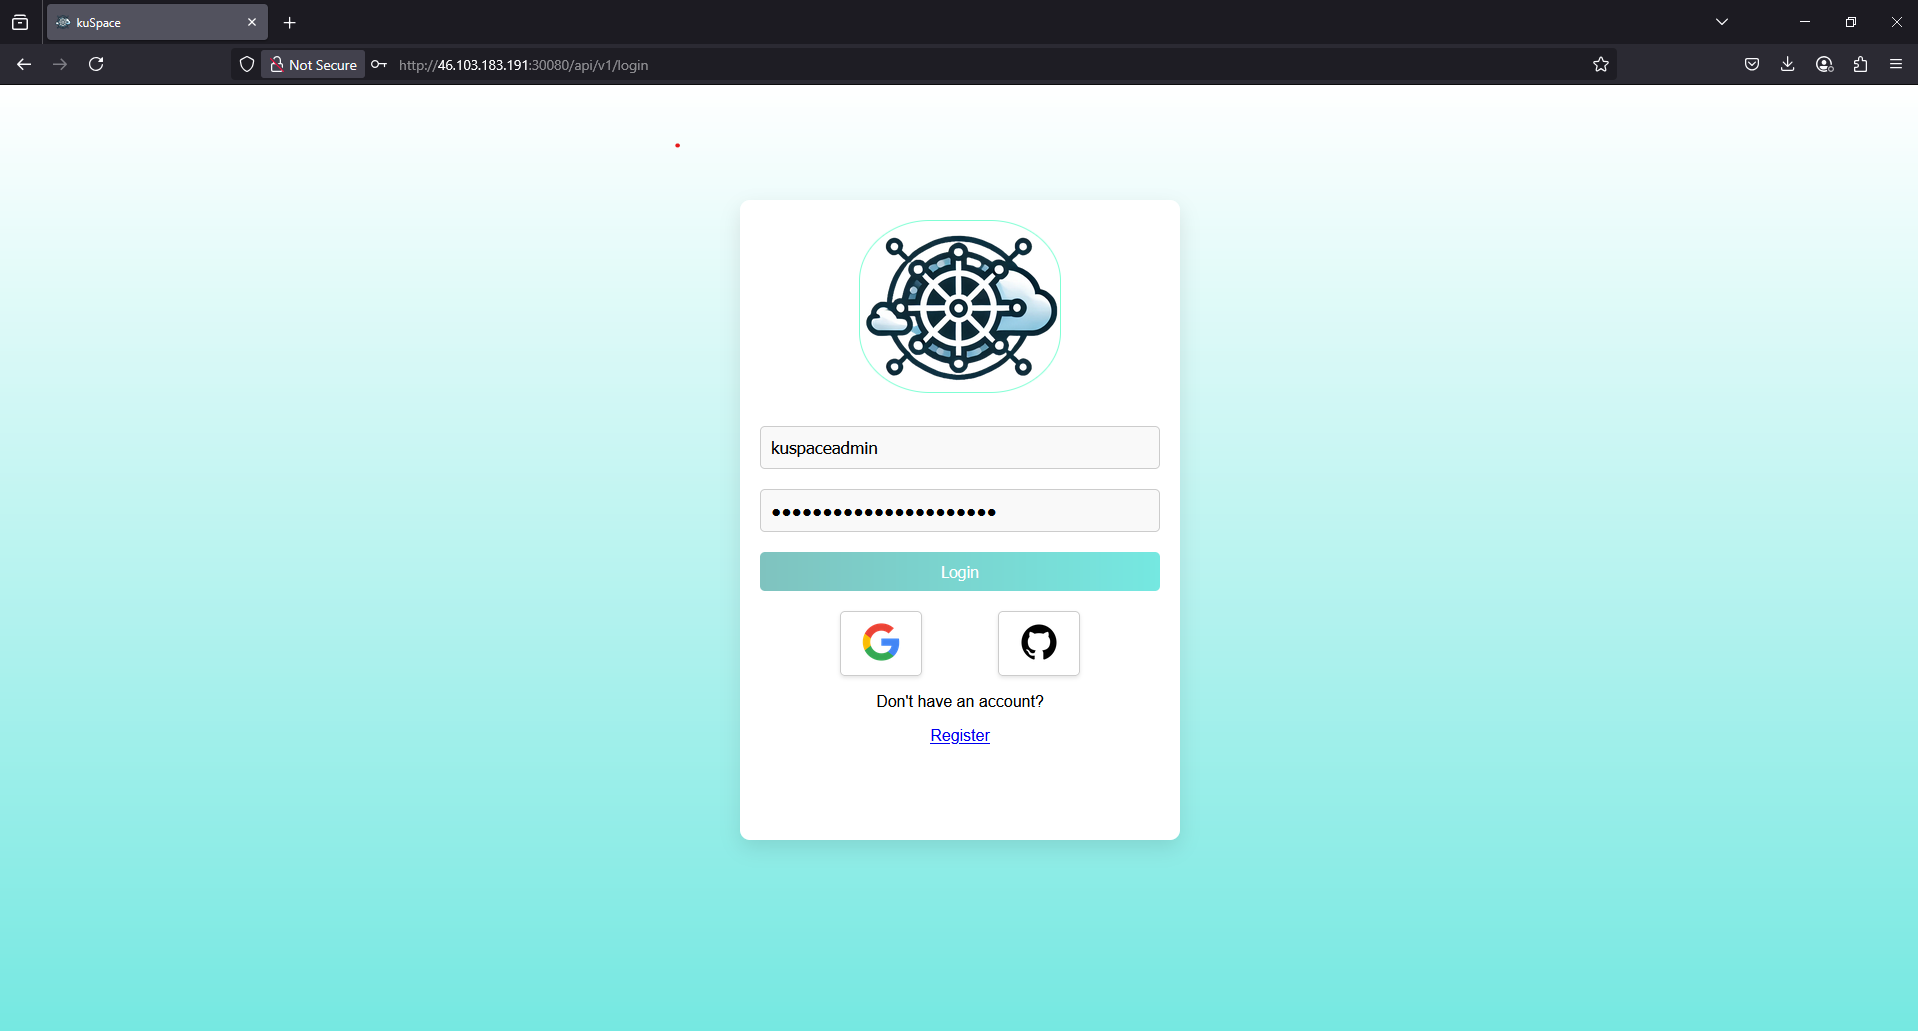
\includegraphics[width=\textwidth]{Images/kuspace_login-page.png}
    \caption{Login Page}
    \label{fig:login}
  \end{subfigure}
  \hfill
  \begin{subfigure}[b]{0.48\textwidth}
    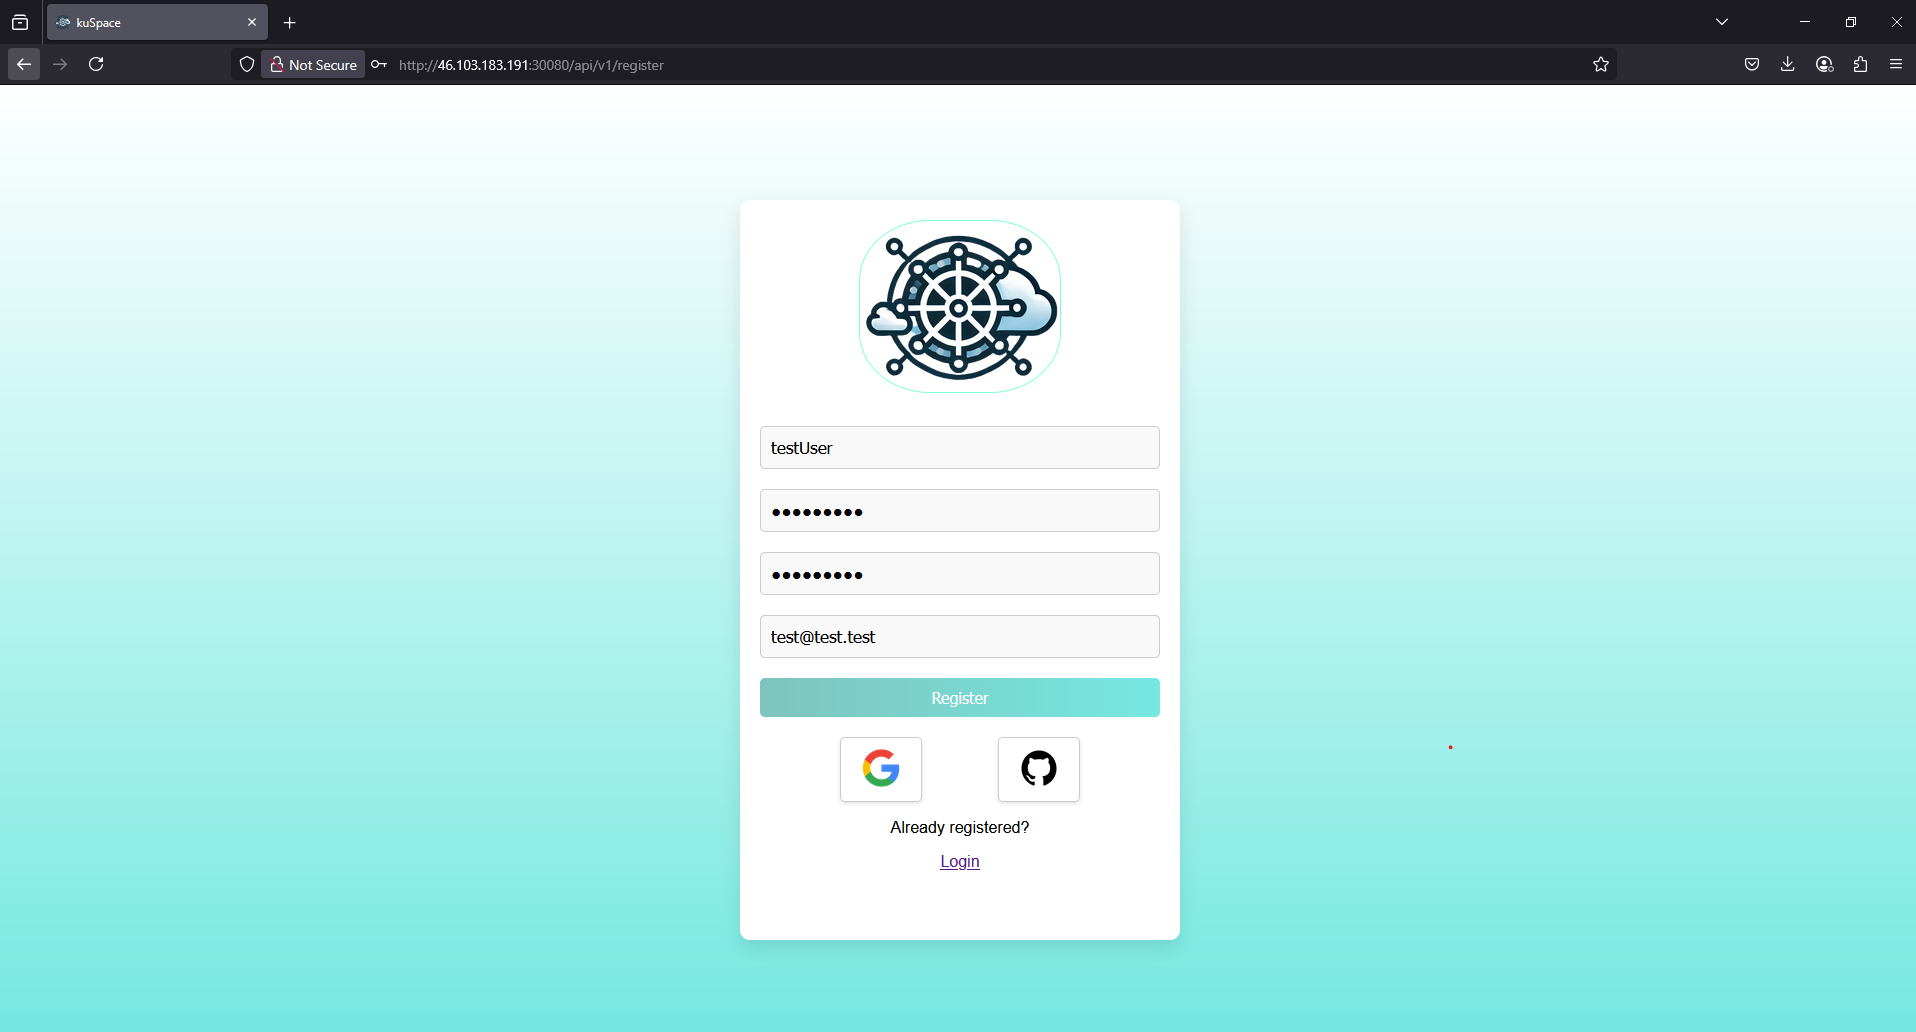
\includegraphics[width=\textwidth]{Images/kuspace_register-page.png}
    \caption{Register Page}
    \label{fig:register}
  \end{subfigure}
  \caption{Kuspace Login and Register Pages}
  \label{fig:authservices}
\end{figure}



The OAuth by Google and Github structure is implemented, yet not fully functional at this point.

There are restrictions on user registration: passwords must match, meet a minimum length, and contain a variety of character types.
Usernames are also constrained by minimum and maximum length requirements, and certain names are prohibited.
\newpage

\subsection{User Perspective}

\begin{figure}[!htbp]
    \centering
    % First row - two side-by-side
    \begin{subfigure}[b]{0.48\textwidth}
        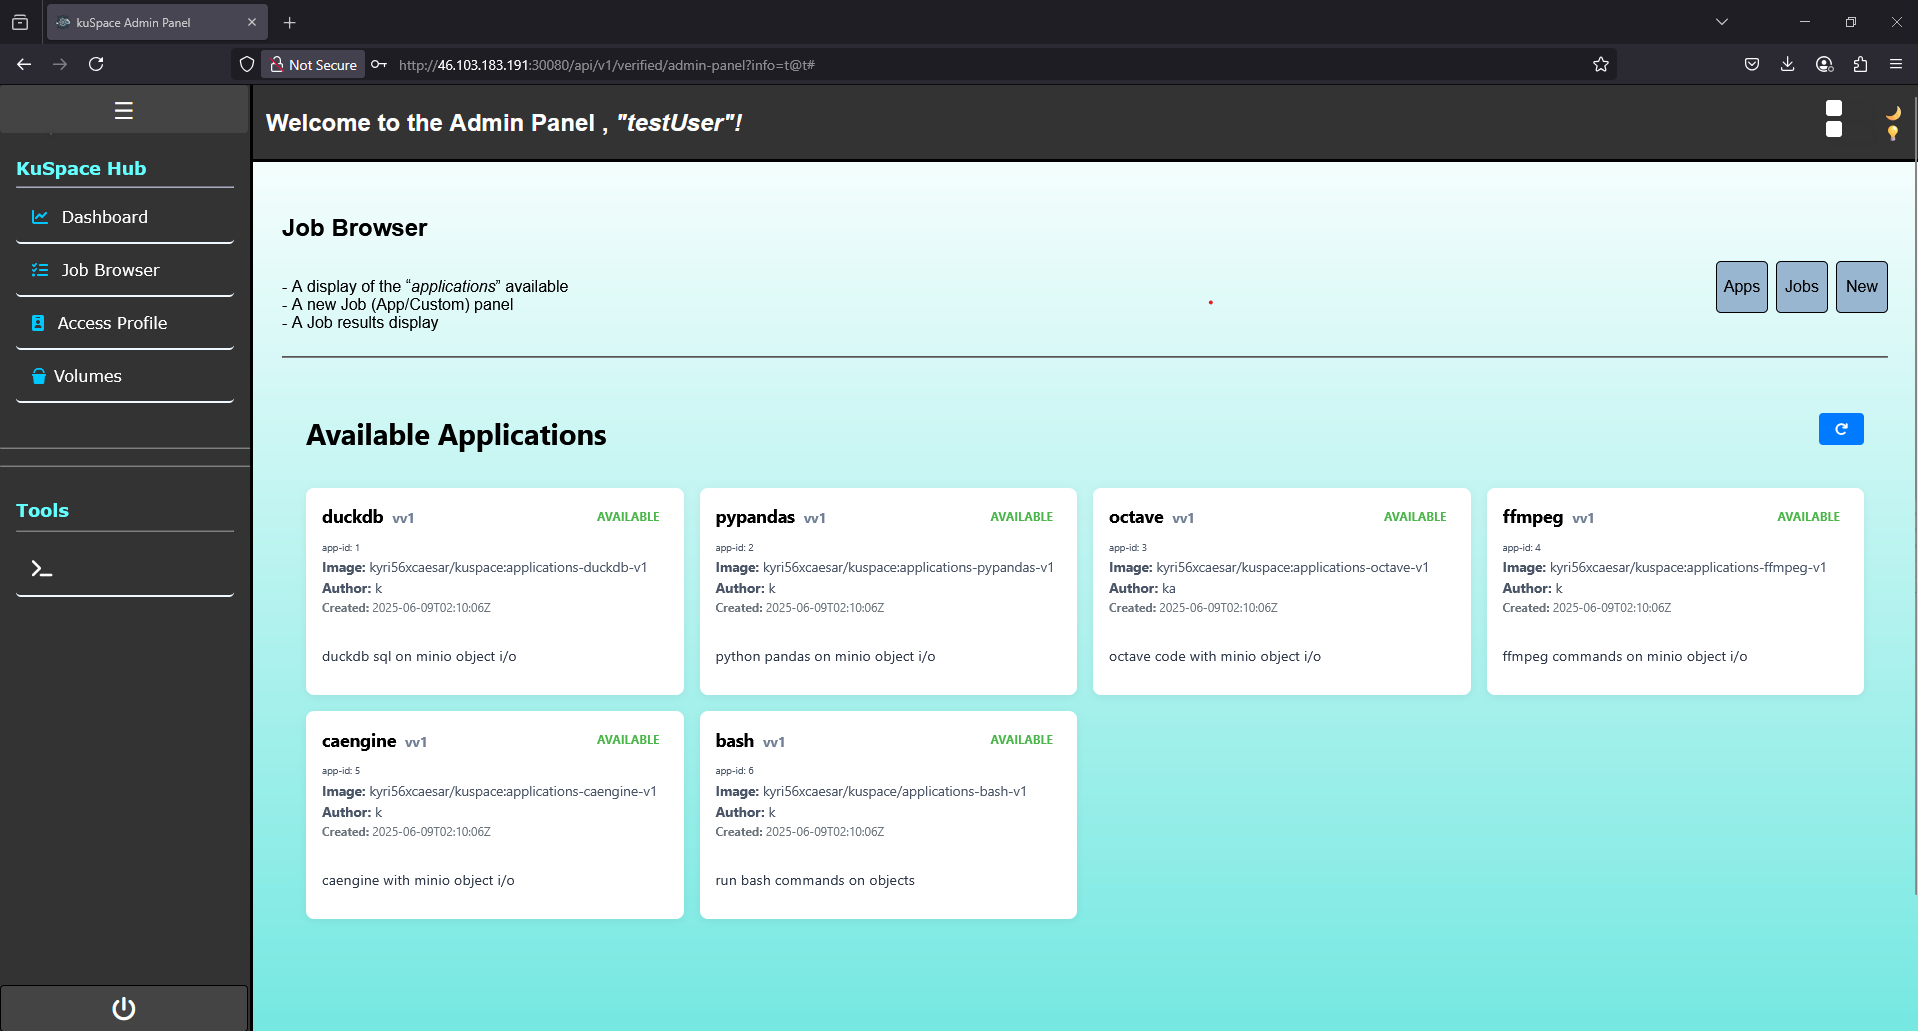
\includegraphics[width=\textwidth]{Images/kuspace_user_jobBrowser_apps.png}
        \caption{Job Browser and App Selection}
        \label{fig:jobbrowserapps}
    \end{subfigure}
    \hfill
    \begin{subfigure}[b]{0.48\textwidth}
        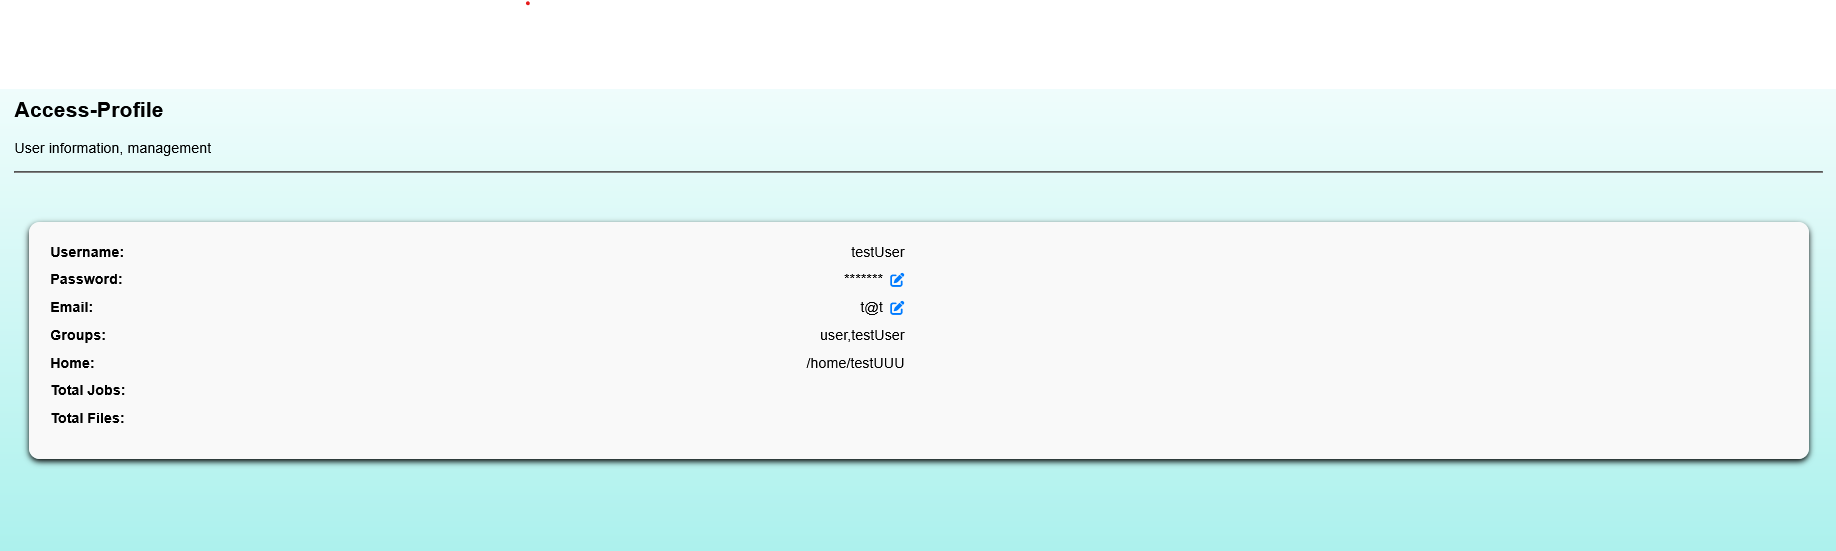
\includegraphics[width=\textwidth]{Images/kuspace_user_accessInfo_change.png}
        \caption{Access Info and Change View}
        \label{fig:accessinfochange}
    \end{subfigure}

    \vspace{1em}

    % Second row - full width
    \begin{subfigure}[b]{0.98\textwidth}
        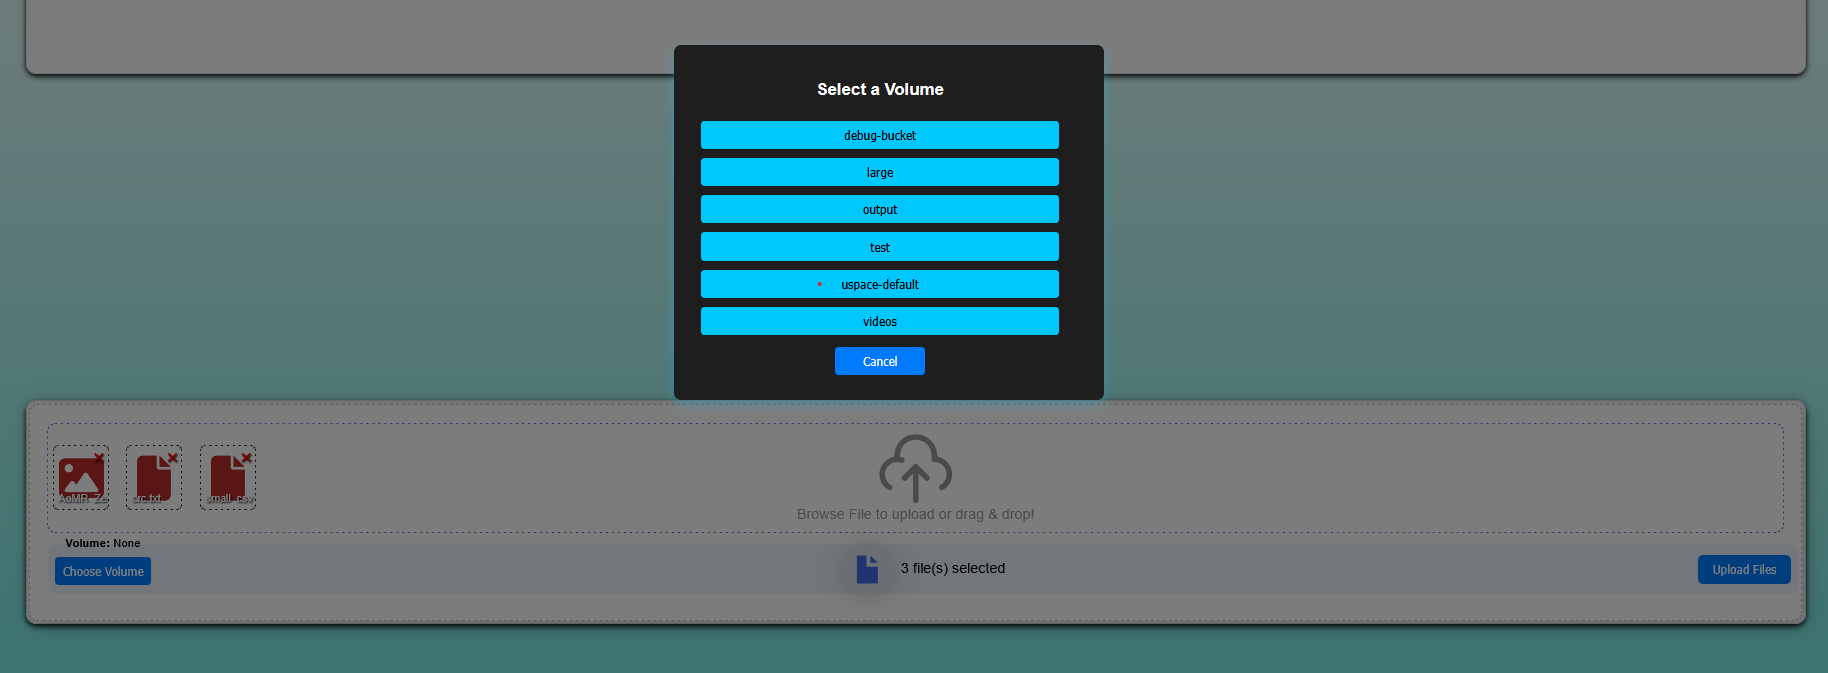
\includegraphics[width=\textwidth]{Images/kuspace_user_fileUploadVolumeChoice.png}
        \caption{File Upload with Volume Selection}
        \label{fig:fileuploadvolume}
    \end{subfigure}

    \caption{User Interface Actions in Kuspace}
    \label{fig:useractions}
\end{figure}

Here we can see the agency a user has to change his credentials, upload files on existing volumes 
and see the available applications. 

\newpage
\begin{figure}[!htbp]
    \centering
    \begin{subfigure}[b]{0.48\textwidth}
        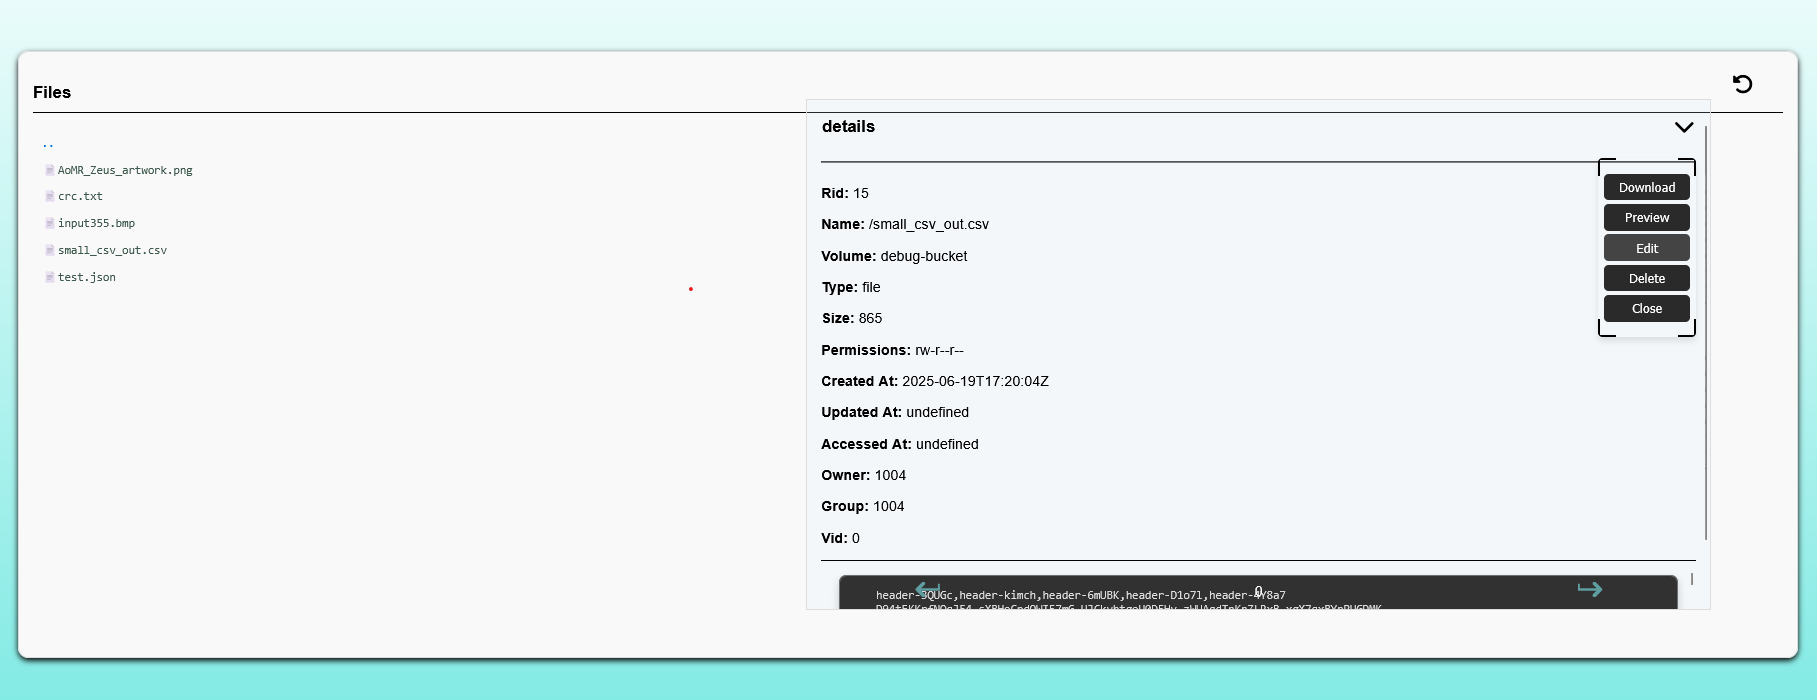
\includegraphics[width=\textwidth]{Images/kuspace_user_fileTraversanlOptions.png}
        \caption{File Traversal and Options}
        \label{fig:filetraversal}
    \end{subfigure}
    \hfill
    \begin{subfigure}[b]{0.48\textwidth}
        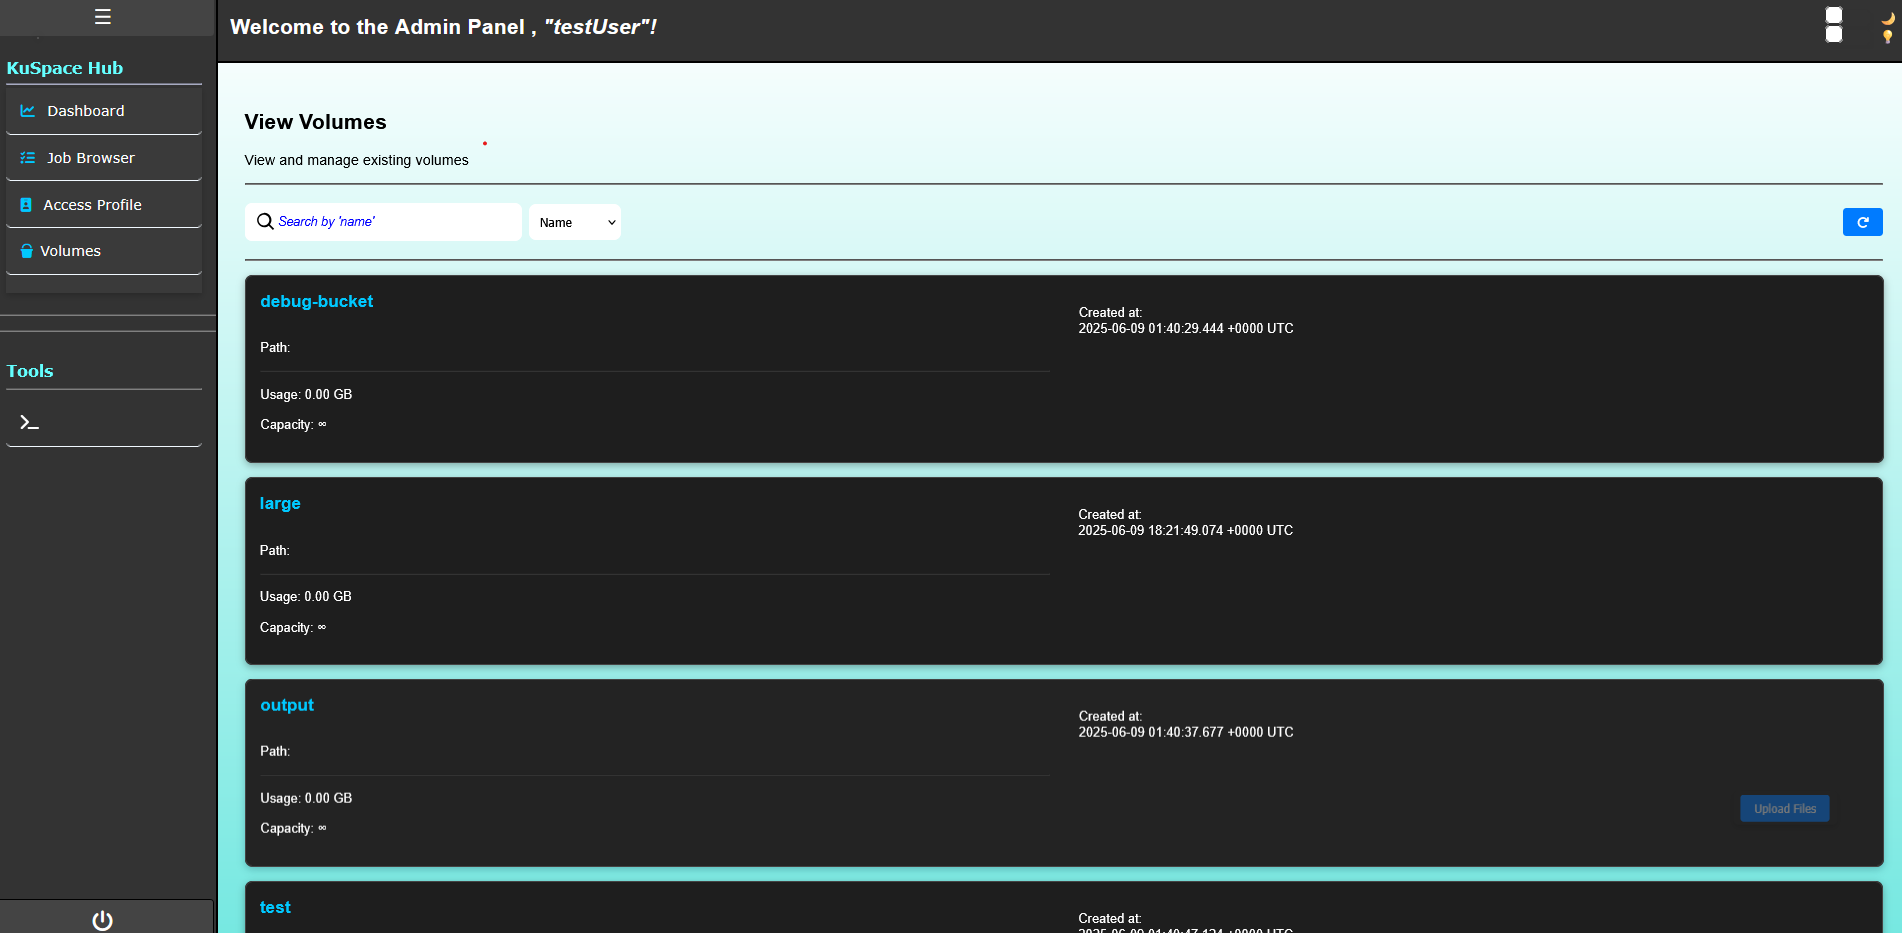
\includegraphics[width=\textwidth]{Images/kuspace_VolumeView.png}
        \caption{Volume Overview}
        \label{fig:volumeview}
    \end{subfigure}
    \caption{Kuspace user views for navigating files and inspecting volumes.}
    \label{fig:user-file-volume}
\end{figure}

\vspace{0.5em}
\noindent
These interfaces allow users to browse directories, inspect resources, and 
understand volume boundaries within the system. Navigation tools and volume 
metadata views help contextualize jobs and uploaded files.


\newpage
\begin{figure}[!htbp]
    \centering
    \begin{subfigure}[b]{0.48\textwidth}
        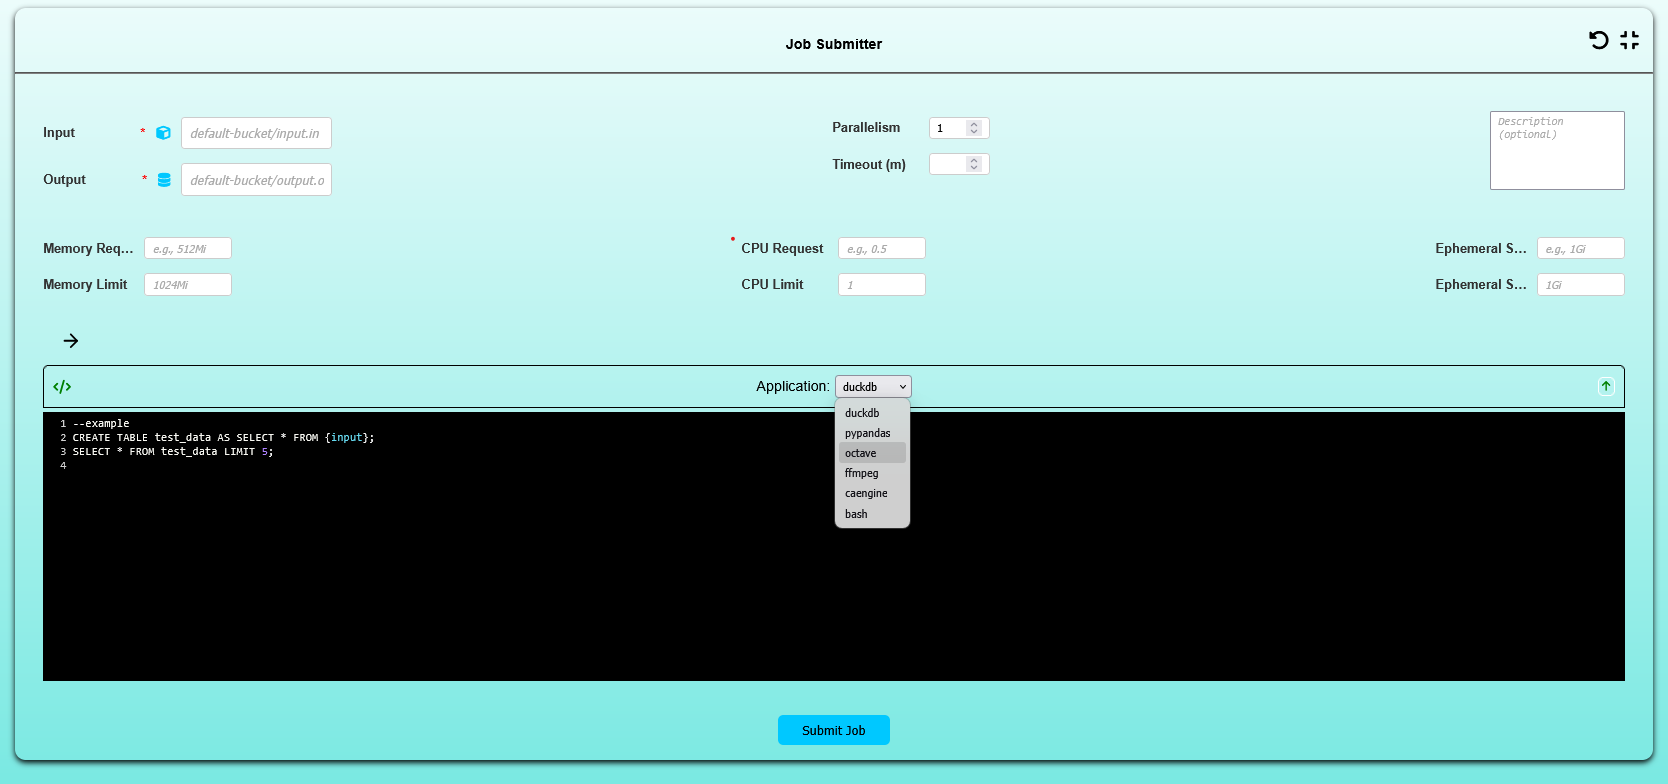
\includegraphics[width=\textwidth]{Images/kuspace_jobSubmitter.png}
        \caption{Job Submitter Panel}
        \label{fig:jobsubmitter}
    \end{subfigure}
    \hfill
    \begin{subfigure}[b]{0.48\textwidth}
        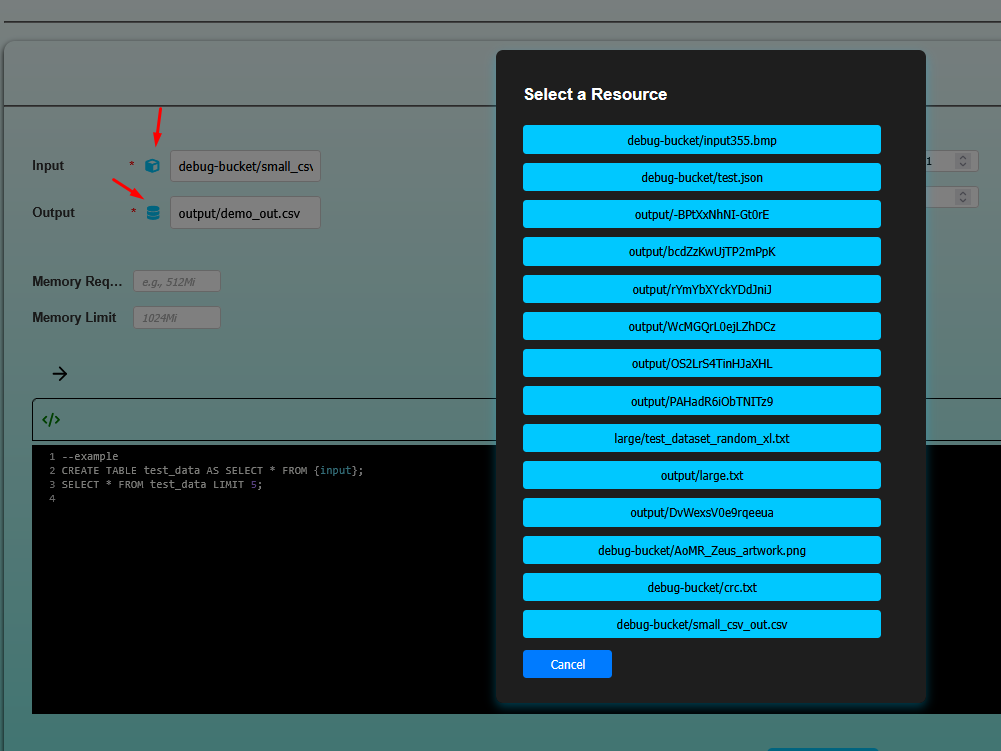
\includegraphics[width=\textwidth]{Images/kuspace_jobSubmitter_selectIO.png}
        \caption{Input/Output Selection}
        \label{fig:jobsubmitterselect}
    \end{subfigure}

    \vspace{1em}

    \begin{subfigure}[b]{0.48\textwidth}
        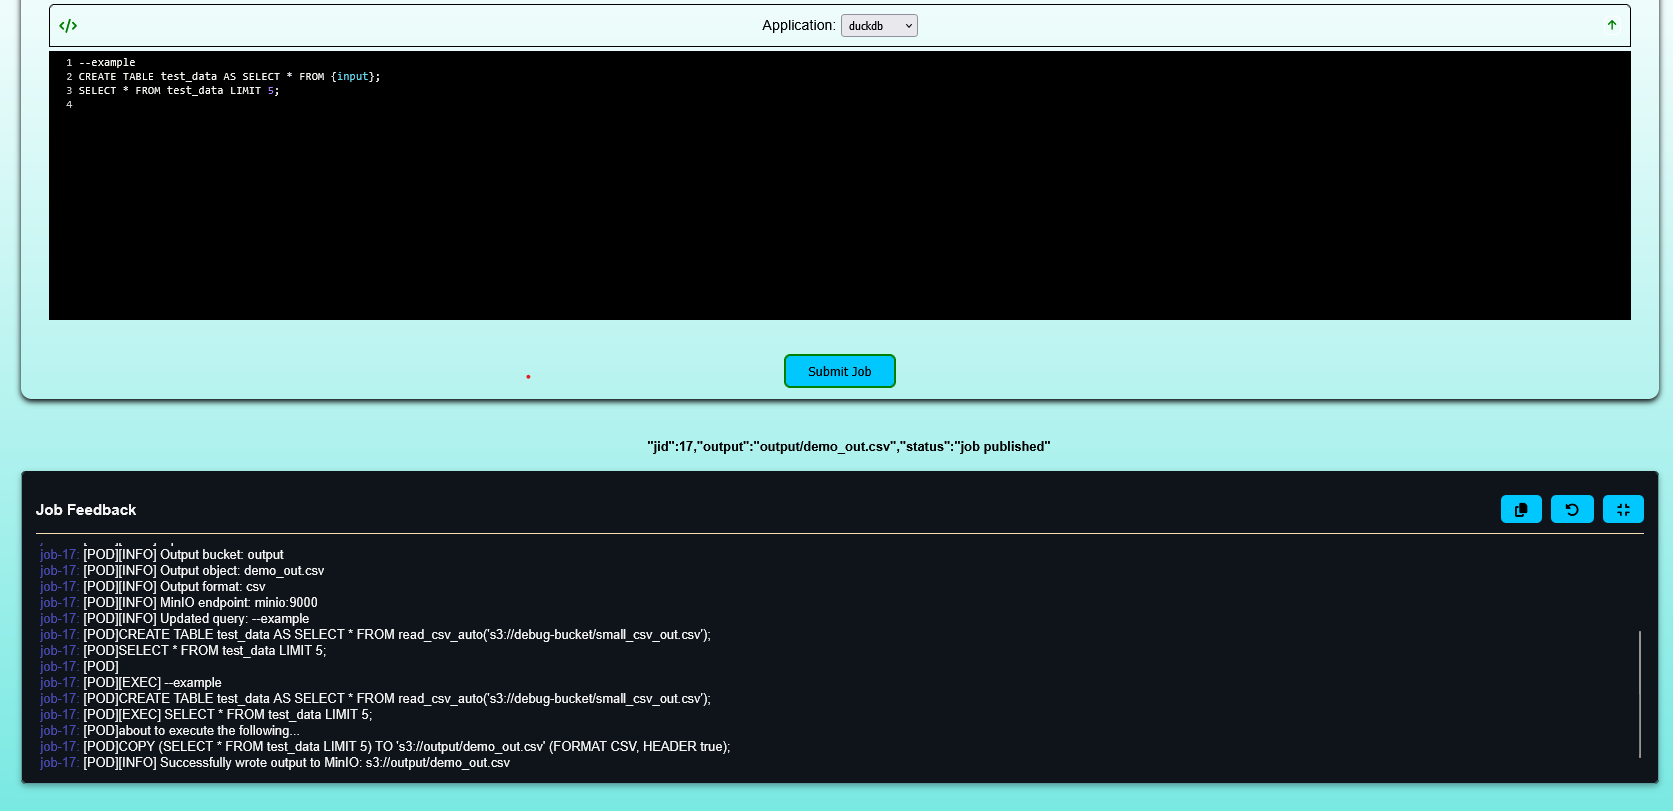
\includegraphics[width=\textwidth]{Images/kuspace_jobSubmission_test.png}
        \caption{Job Published \& Execution Streaming}
        \label{fig:jobsubmission}
    \end{subfigure}
    \hfill
    \begin{subfigure}[b]{0.48\textwidth}
        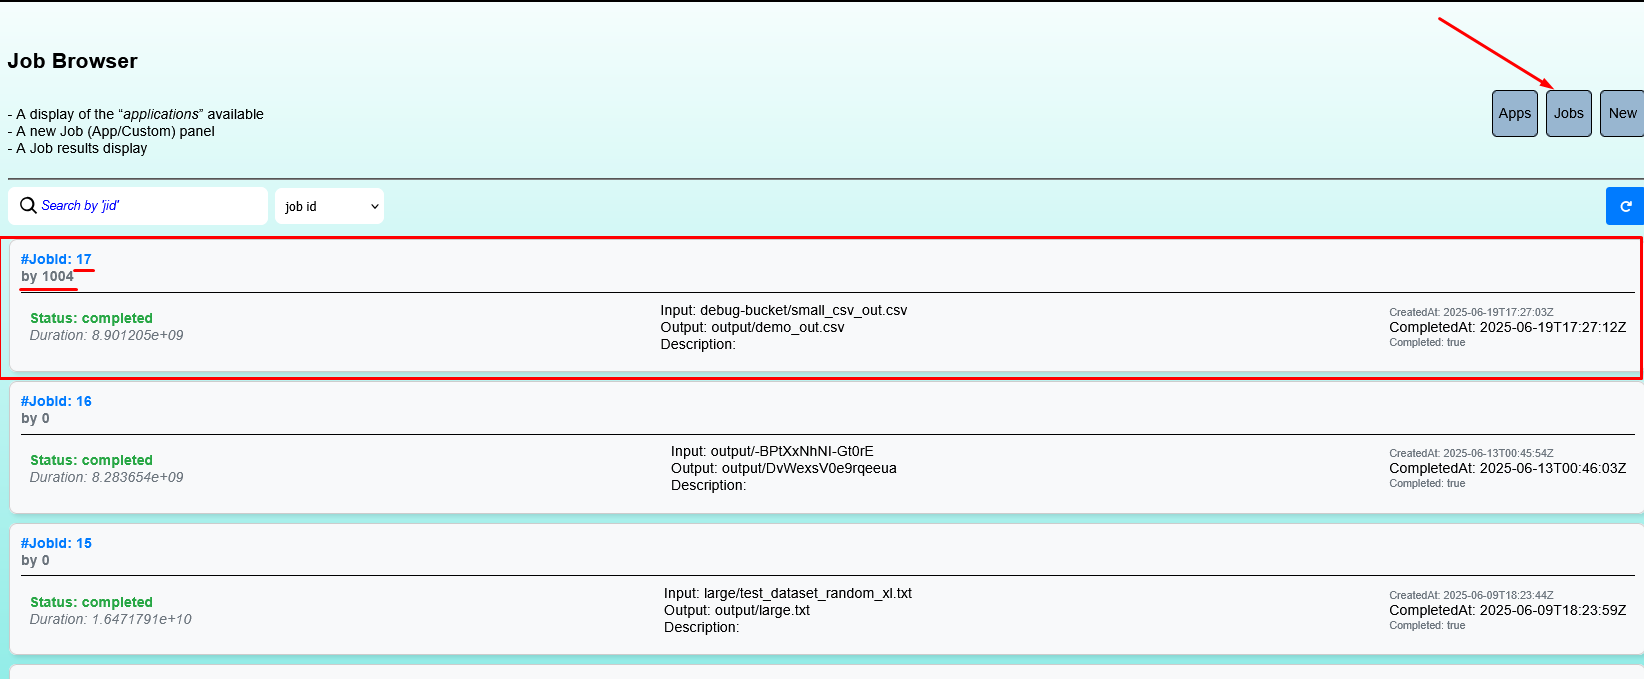
\includegraphics[width=\textwidth]{Images/kuspace_jobView.png}
        \caption{Job Execution Results}
        \label{fig:jobview}
    \end{subfigure}

    \caption{Kuspace user interface for submitting jobs.}
    \label{fig:kuspacejobflow}
\end{figure}

\vspace{0.5em}
\noindent
The workflow includes selecting an application, 
specifying input/output paths, tuning job parameters, 
and viewing results.


\newpage

\subsection{Admin Perspective}
Kuspace advanced administrative actions, including job mutation and system configuration view. 
These tools help define volumes, manage jobs, and manage resource properties.
These views allow administrators to control access and maintain structure.

There are also stylistic options, for example dark-mode, and less verbosity in the top right corner.

\begin{figure}[!htbp]
    \centering
    \begin{subfigure}[b]{0.48\textwidth}
        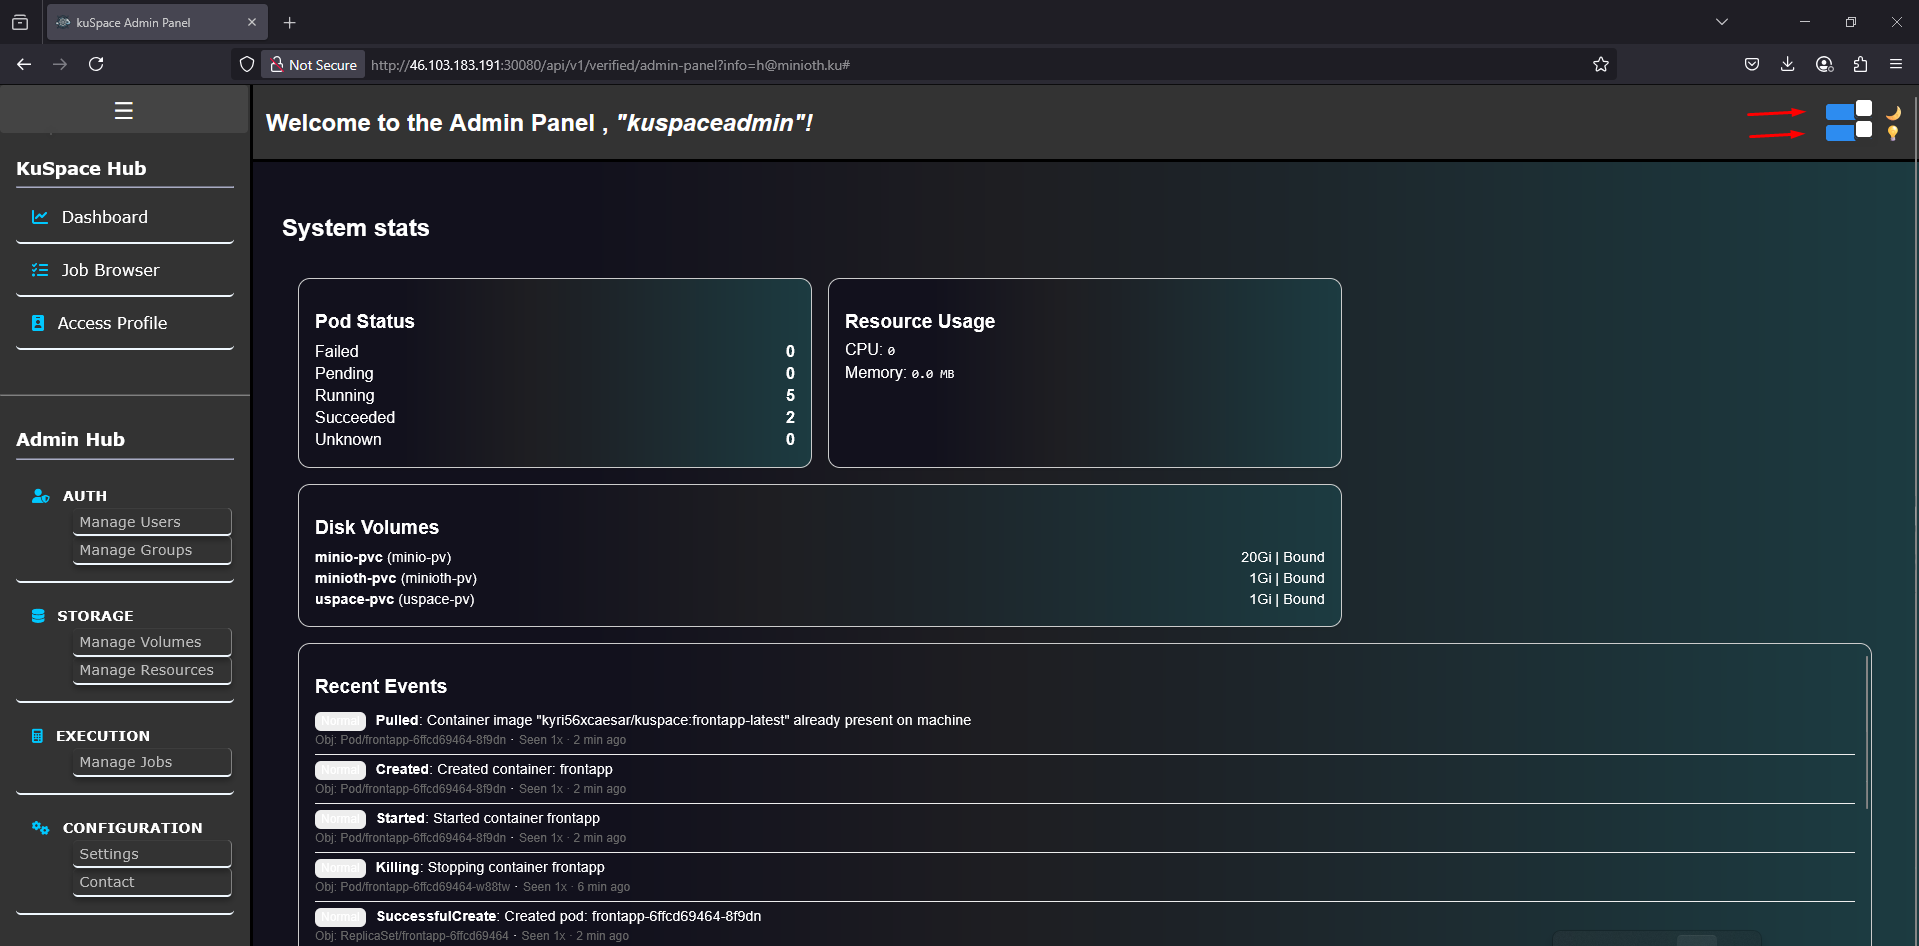
\includegraphics[width=\textwidth]{Images/kuspace_adminDashboard.png}
        \caption{Admin Dashboard Overview}
        \label{fig:adminviewdashboard}
    \end{subfigure}
    \hfill
    \begin{subfigure}[b]{0.48\textwidth}
        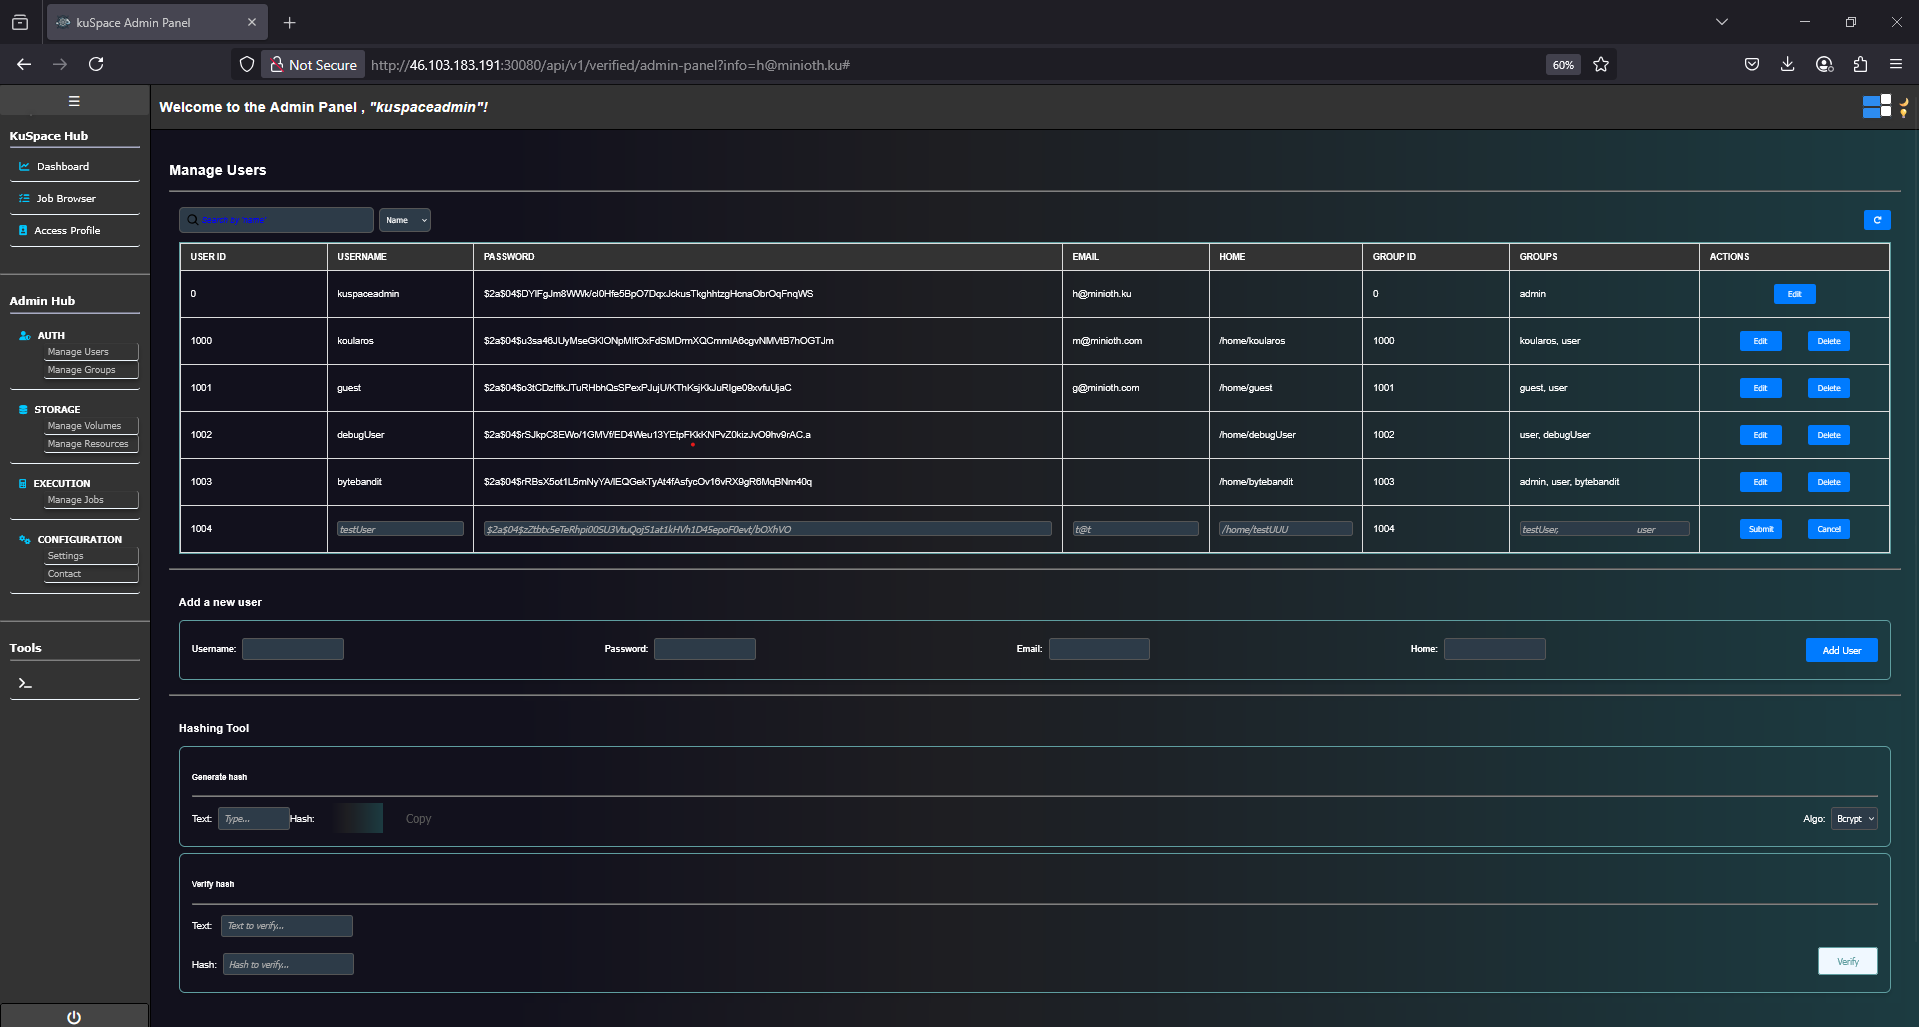
\includegraphics[width=\textwidth]{Images/kuspace_admin_ManageUsers.png}
        \caption{User Management Panel}
        \label{fig:adminmanageusers}
    \end{subfigure}

    \vspace{1em}

    \begin{subfigure}[b]{0.48\textwidth}
        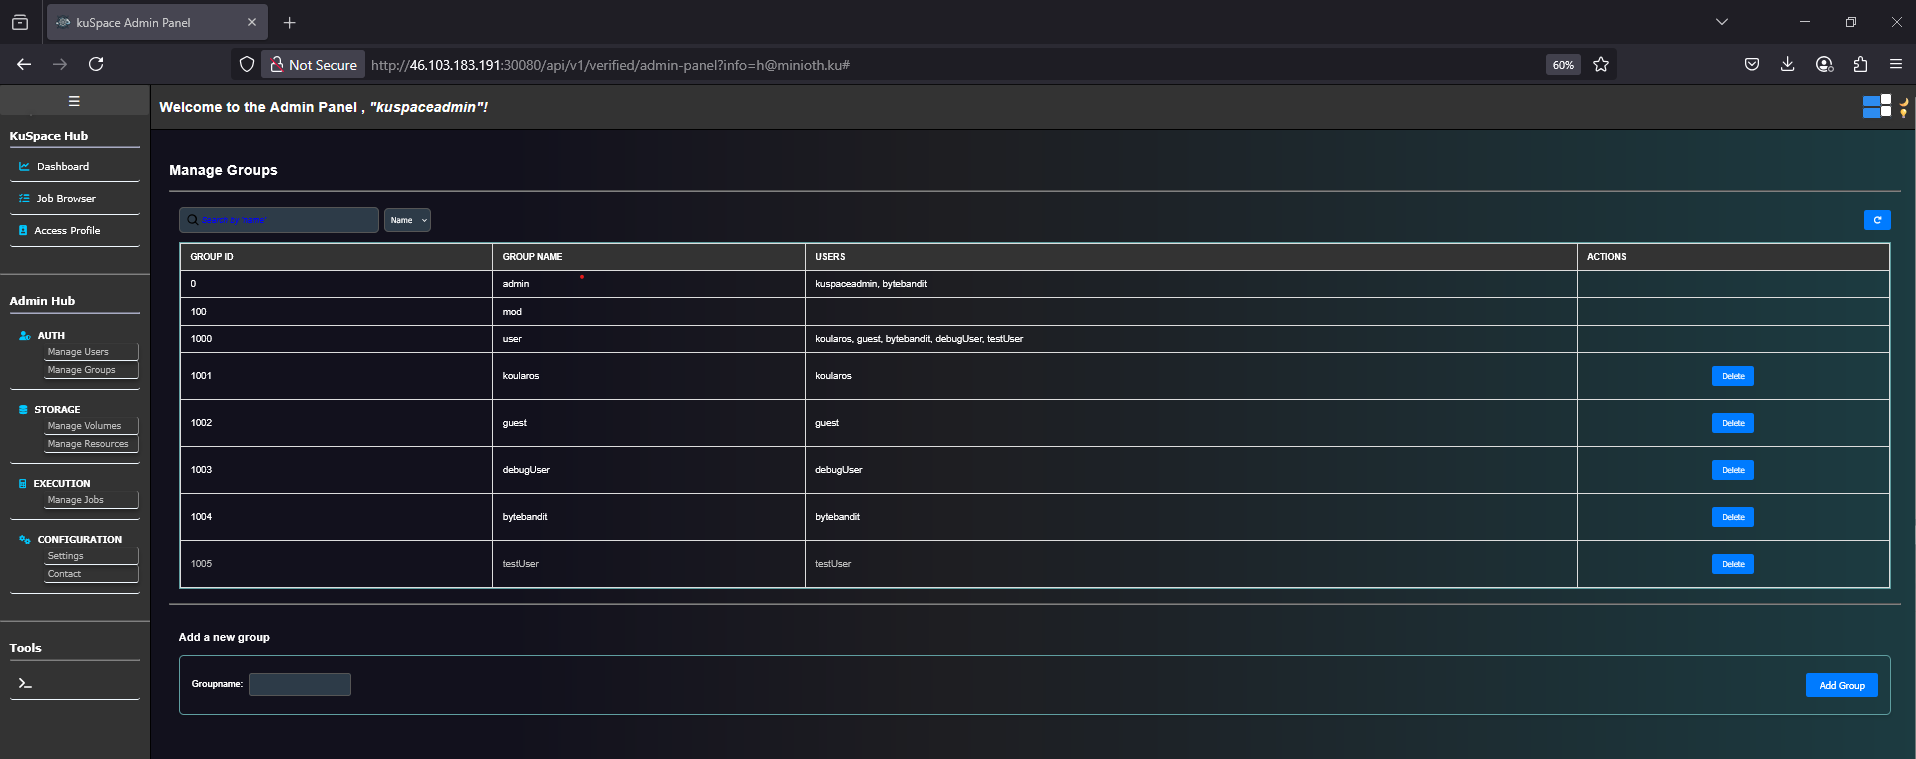
\includegraphics[width=\textwidth]{Images/kuspace_admin_ManageGroups.png}
        \caption{Group Management}
        \label{fig:adminmanagegroups}
    \end{subfigure}
    \hfill
    \begin{subfigure}[b]{0.48\textwidth}
        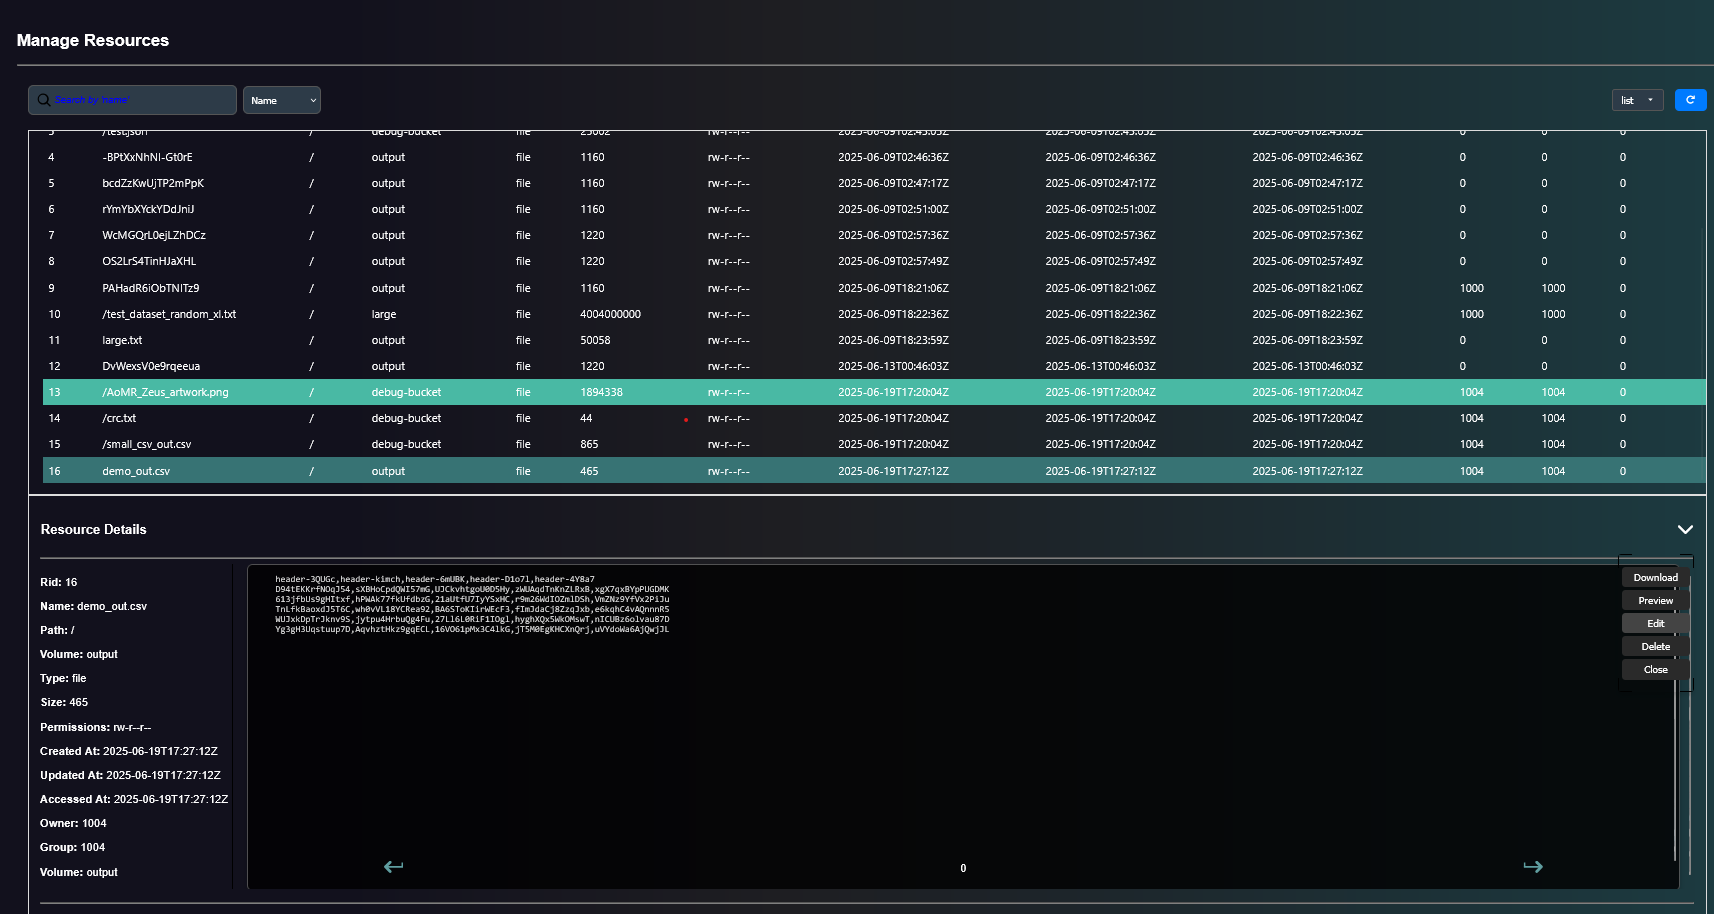
\includegraphics[width=\textwidth]{Images/kuspace_admin_ManageResources.png}
        \caption{Resources Management}
        \label{fig:adminmanageresources}
    \end{subfigure}

    \caption{Kuspace admin interface for managing users, groups, and resources.}
\end{figure}
\vspace{0.5em}
\noindent

\vspace{1em}

\begin{figure}[!htbp]
    \centering
    \begin{subfigure}[b]{0.48\textwidth}
        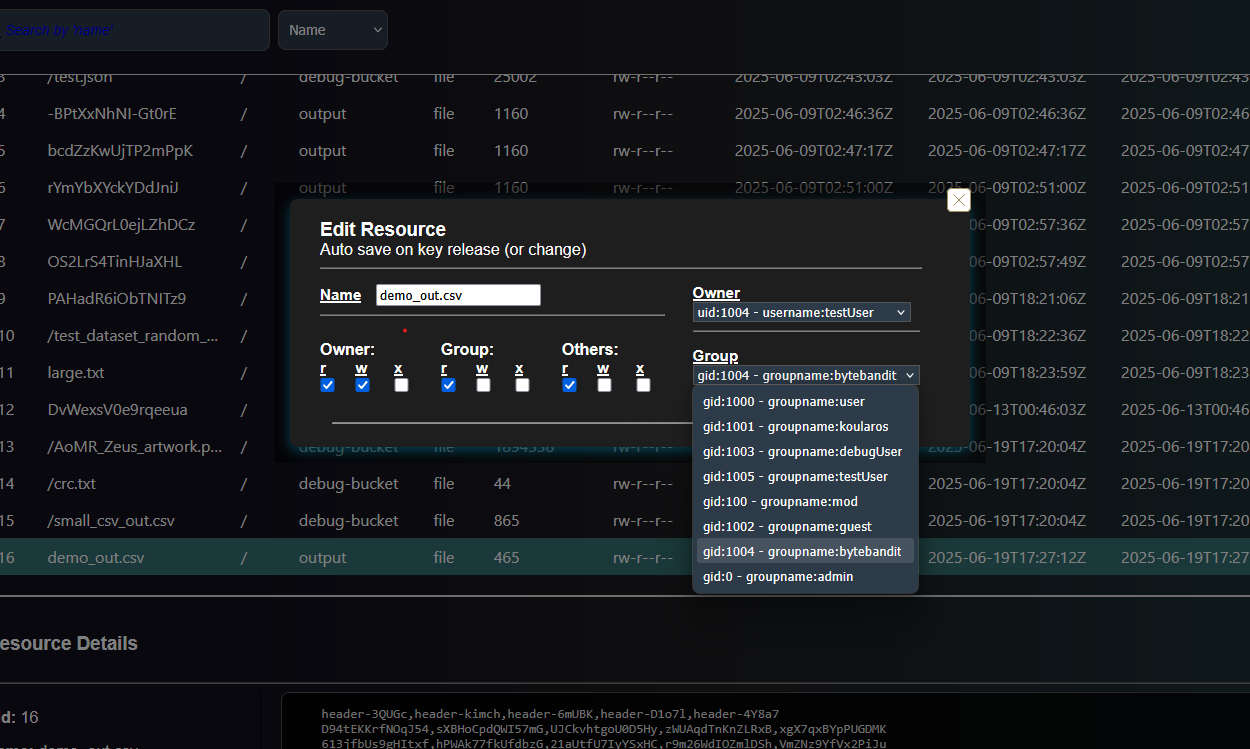
\includegraphics[width=\textwidth]{Images/kuspace_admin_EditResource.png}
        \caption{Edit Resource Metadata}
        \label{fig:admineditresource}
    \end{subfigure}
    \hfill
    \begin{subfigure}[b]{0.48\textwidth}
        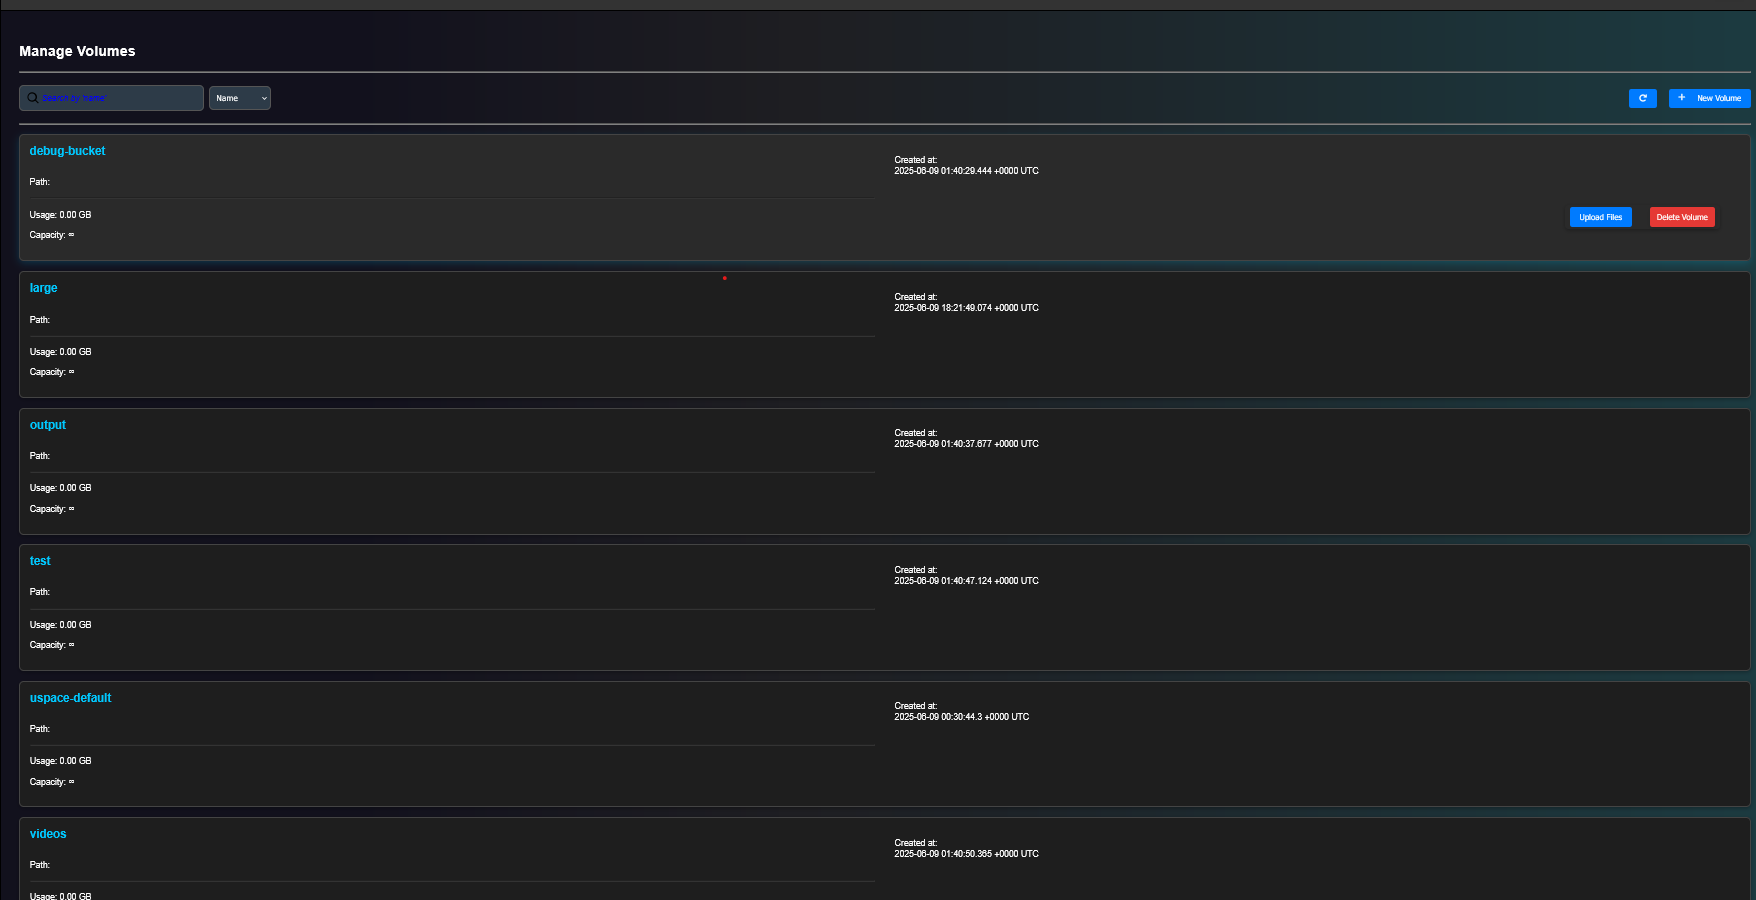
\includegraphics[width=\textwidth]{Images/kuspace_admin_ManageVolumes.png}
        \caption{Volume Overview}
        \label{fig:adminmanagevolumes}
    \end{subfigure}

    \vspace{1em}

    \begin{subfigure}[b]{0.48\textwidth}
        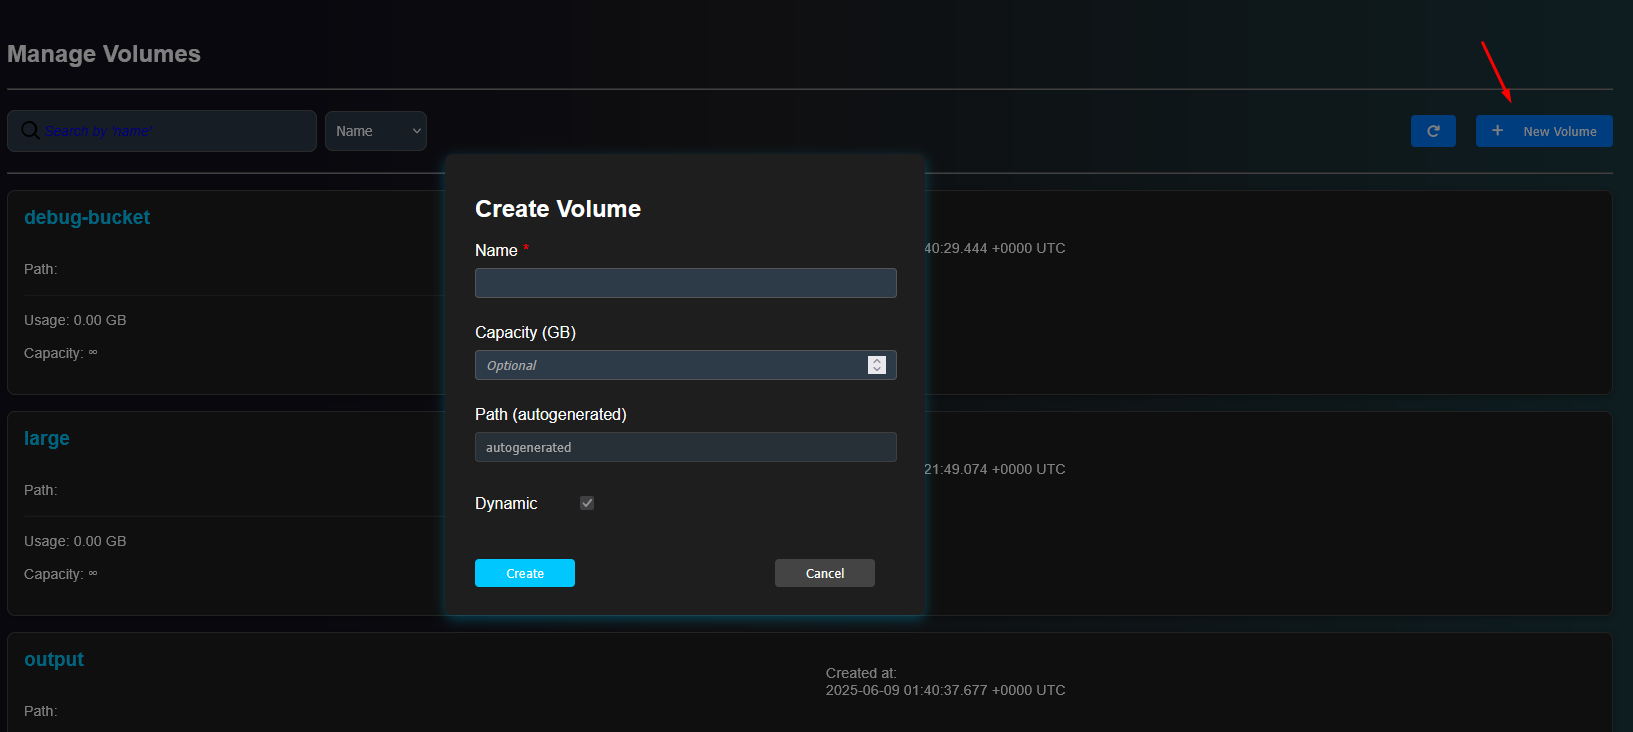
\includegraphics[width=\textwidth]{Images/kuspace_admin_CreateVolume.png}
        \caption{Create New Volume}
        \label{fig:admincreatevolume}
    \end{subfigure}
    \hfill
    \begin{subfigure}[b]{0.48\textwidth}
        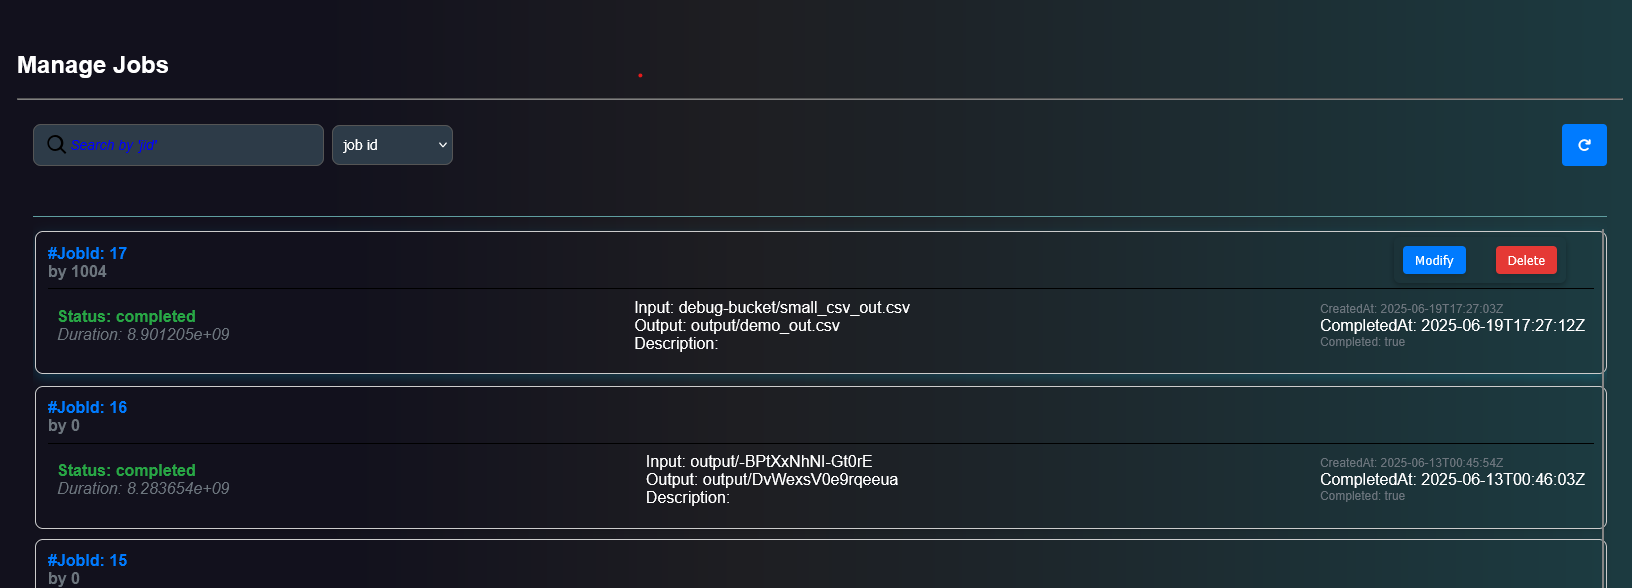
\includegraphics[width=\textwidth]{Images/kuspace_admin_ManageJobs.png}
        \caption{Manage Jobs}
        \label{fig:adminmanagejobs}
    \end{subfigure}

    \vspace{1em}

    \centering
    \begin{subfigure}[b]{0.48\textwidth}
        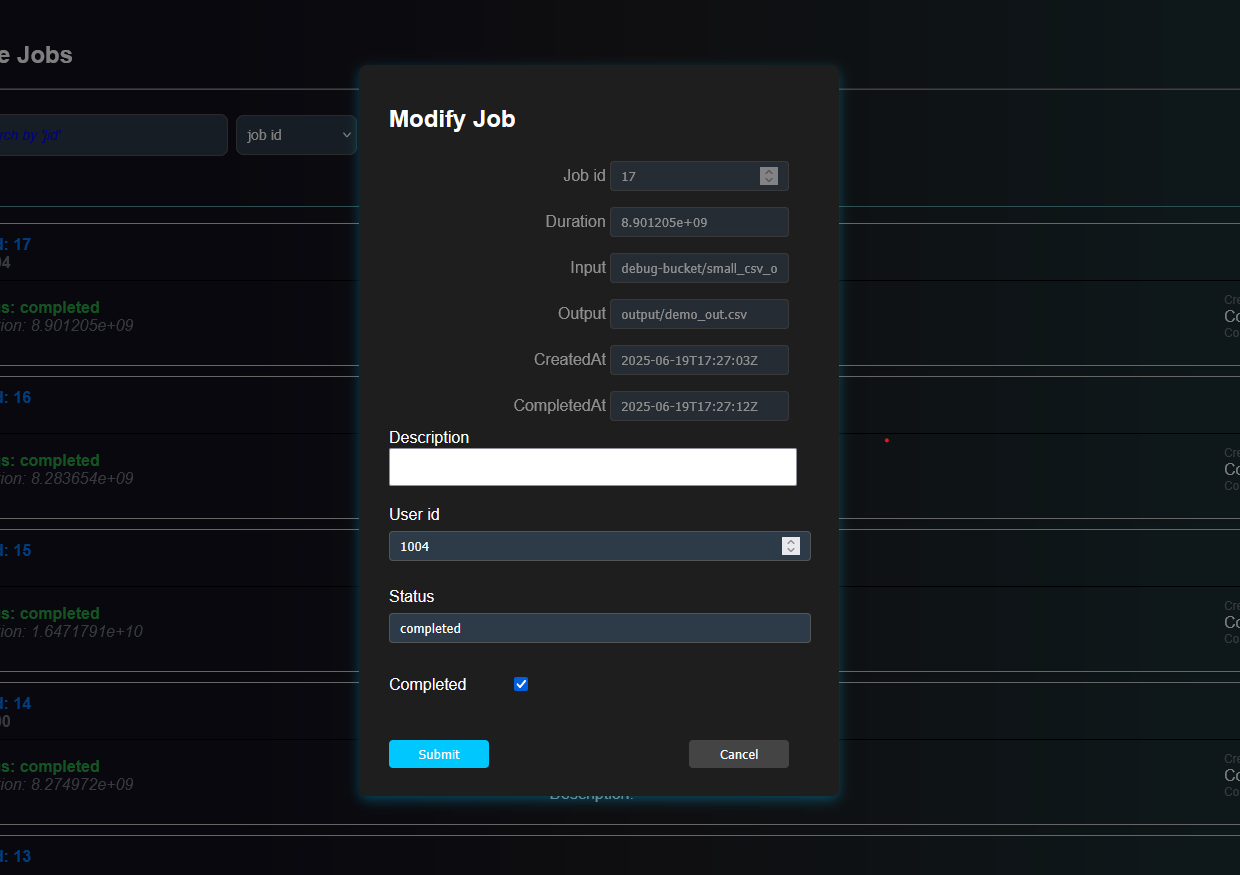
\includegraphics[width=\textwidth]{Images/kuspace_admin_ModifyJob.png}
        \caption{Modify Submitted Job}
        \label{fig:adminmodifyjob}
    \end{subfigure}
    \hfill
    \begin{subfigure}[b]{0.48\textwidth}
        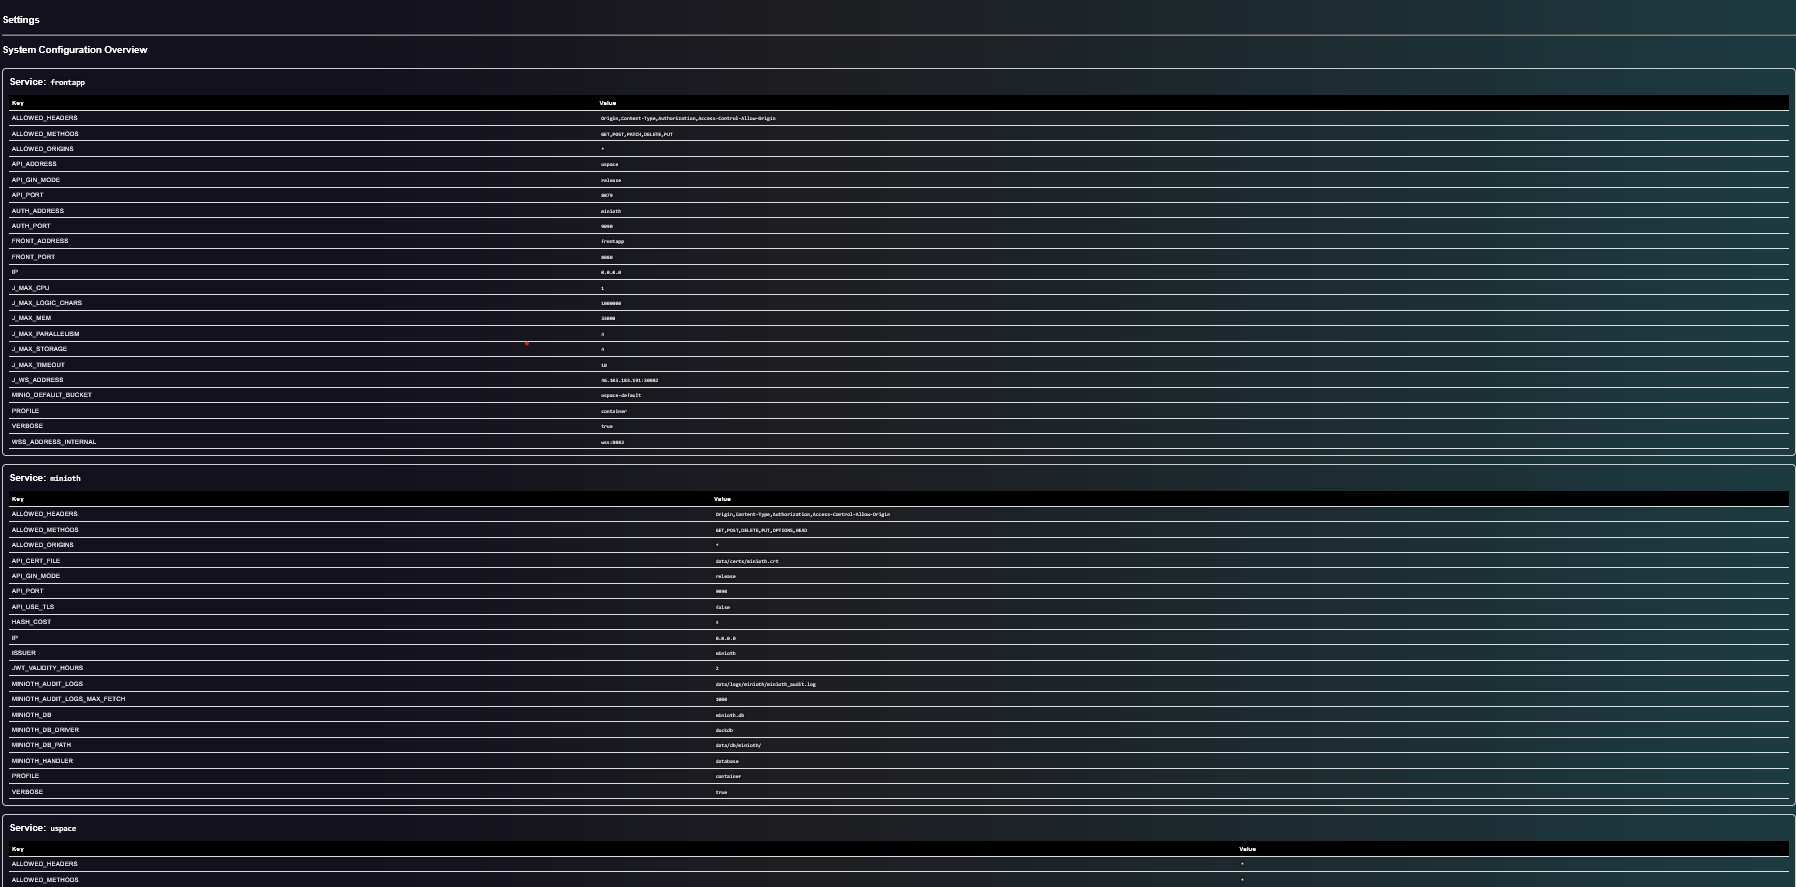
\includegraphics[width=\textwidth]{Images/kuspace_admin_Settings.png}
        \caption{Settings Panel}
        \label{fig:adminsettings}
    \end{subfigure}
    \caption{Kuspace admin views for storage and job management.}
\end{figure}
\vspace{0.5em}
\noindent


\newpage
\subsection{Job Examples}

In this section, we demonstrate two distinct job examples that showcase the system's ability to execute containerized applications over uploaded data:

\begin{itemize}
    \item A \textbf{Bash-based job} that counts the number of occurrences of the string \texttt{"bash"} within a 4GB file of random characters.
    \item A \textbf{DuckDB-based job} that computes a histogram of the first character of each line in a structured text file.
\end{itemize}

\subsubsection*{Example 1: Bash Job – Count Occurrences}

The input file consists of 4GB of random characters including the word \texttt{"bash"} scattered throughout.

\paragraph{Job Logic:}
\begin{verbatim}
grep -o 'bash' input.txt | wc -l
\end{verbatim}

\paragraph{Result:}  
\texttt{254} occurrences of \texttt{"bash"} were found.

This result can be verified locally using a terminal or text editor (assuming sufficient memory).

\begin{figure}[!htbp]
    \centering
    \begin{subfigure}[b]{0.9\textwidth}
        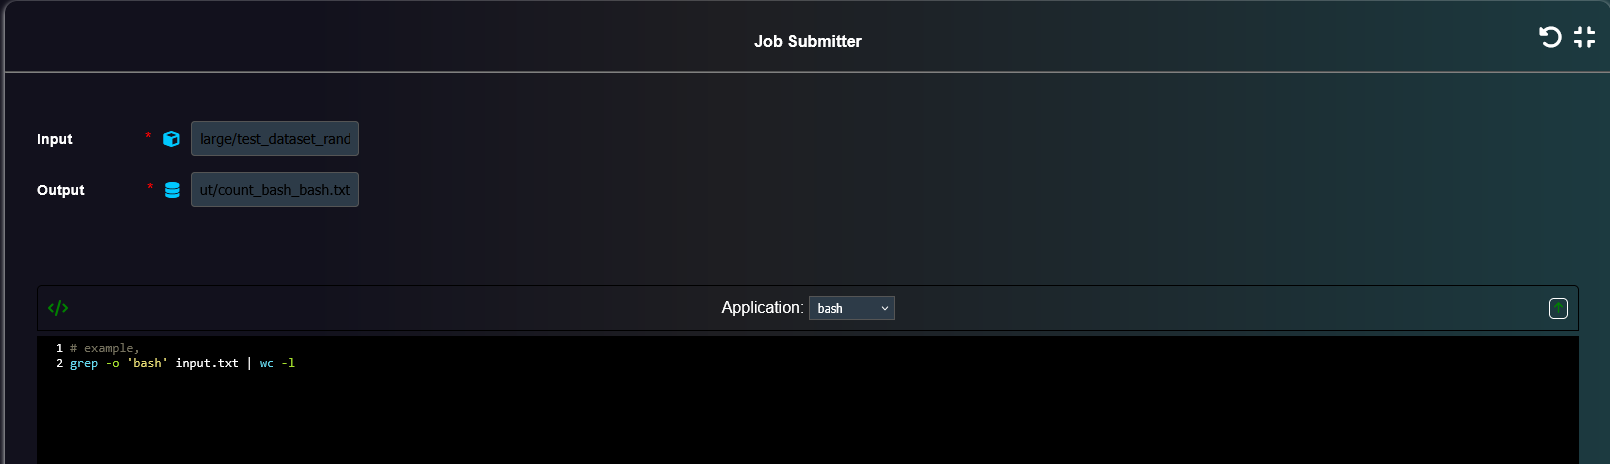
\includegraphics[width=\textwidth]{Images/bash_count_example.txt.png}
        \caption{Bash App job logic submitted via UI}
        \label{fig:examplebash1.1}
    \end{subfigure}

    \vspace{1em}

    \begin{subfigure}[b]{0.9\textwidth}
        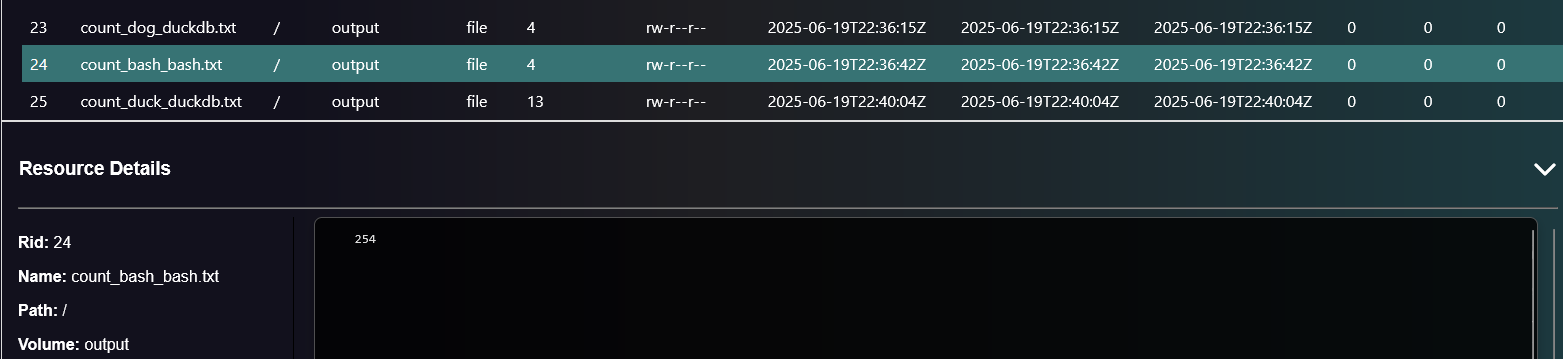
\includegraphics[width=\textwidth]{Images/bash_count_result.png}
        \caption{Bash App job output}
        \label{fig:examplebash1.2}
    \end{subfigure}

    \vspace{1em}

    \begin{subfigure}[b]{0.9\textwidth}
        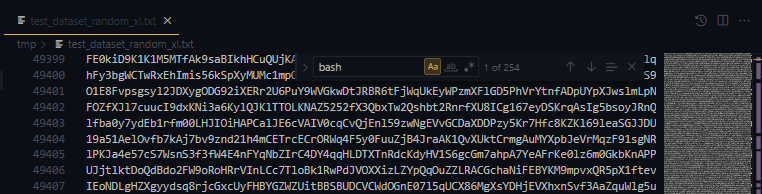
\includegraphics[width=\textwidth]{Images/bash_count.txt.png}
        \caption{Manual result verification (e.g., via editor)}
        \label{fig:examplebash1.3}
    \end{subfigure}
    \caption{Bash job: Counting occurrences of a word in a large file}
\end{figure}

\newpage
\subsubsection*{Example 2: DuckDB Job – Line Start Histogram}

This job uses a smaller text file to illustrate SQL capabilities more clearly. Each line in the file starts with a capital letter forming the line:

\begin{quote}
\texttt{DUCKDBBASHOCTAVE}
\end{quote}

\paragraph{Job Logic:}
\begin{verbatim}
CREATE TABLE lines AS SELECT * FROM {input};

SELECT substr(column0, 1, 1) AS first_char, count(*) AS line_count
FROM lines
GROUP BY first_char
ORDER BY line_count DESC;
\end{verbatim}

\paragraph{Result:}

\begin{verbatim}
D,2
C,2
B,2
A,2
U,1
K,1
S,1
H,1
O,1
T,1
V,1
E,1
\end{verbatim}

As expected, each starting letter is counted accurately and returned in descending order of frequency.

\begin{figure}[!htbp]
    \centering
    \begin{subfigure}[b]{0.9\textwidth}
        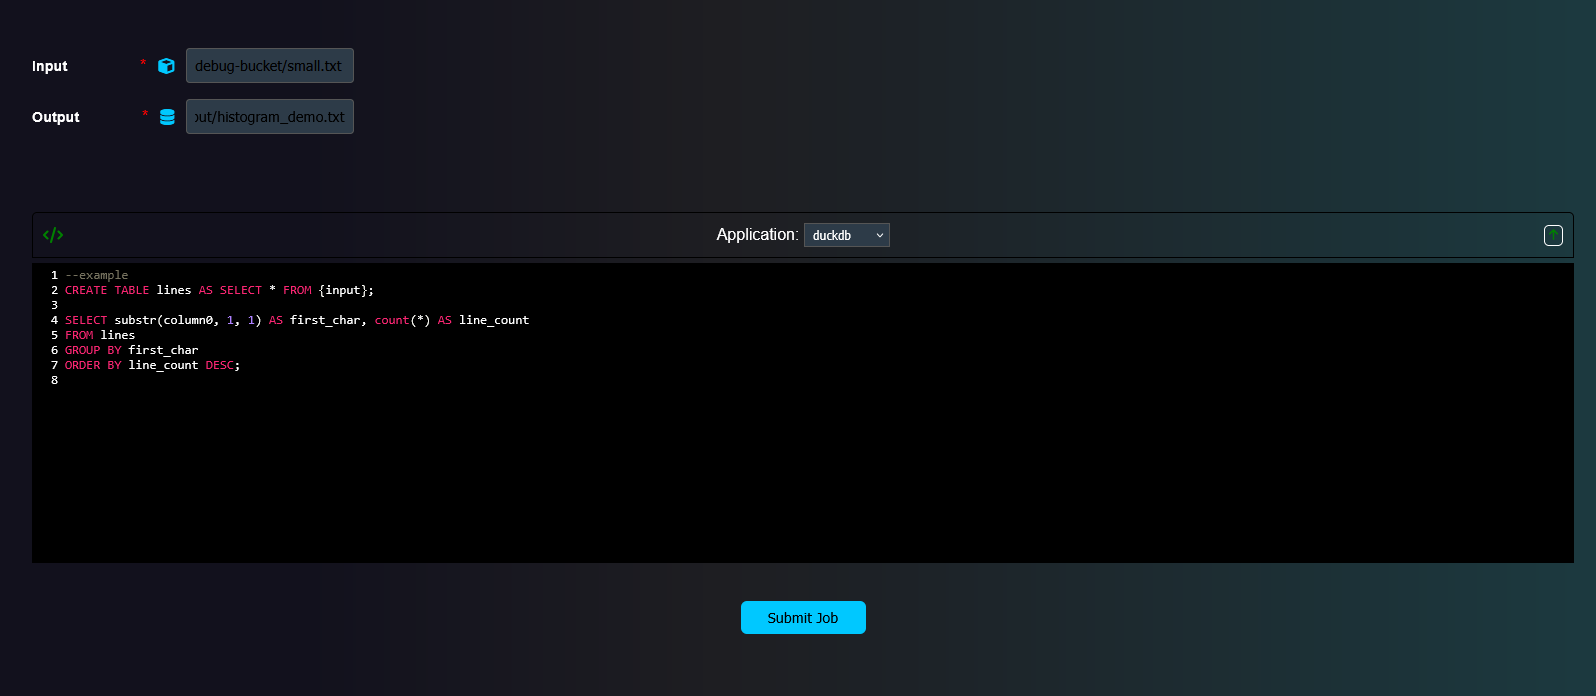
\includegraphics[width=\textwidth]{Images/duckdb_histogram_demo.png}
        \caption{DuckDB job query and configuration}
        \label{fig:exampleduckdb.1}
    \end{subfigure}

    \vspace{1em}

    \begin{subfigure}[b]{0.9\textwidth}
        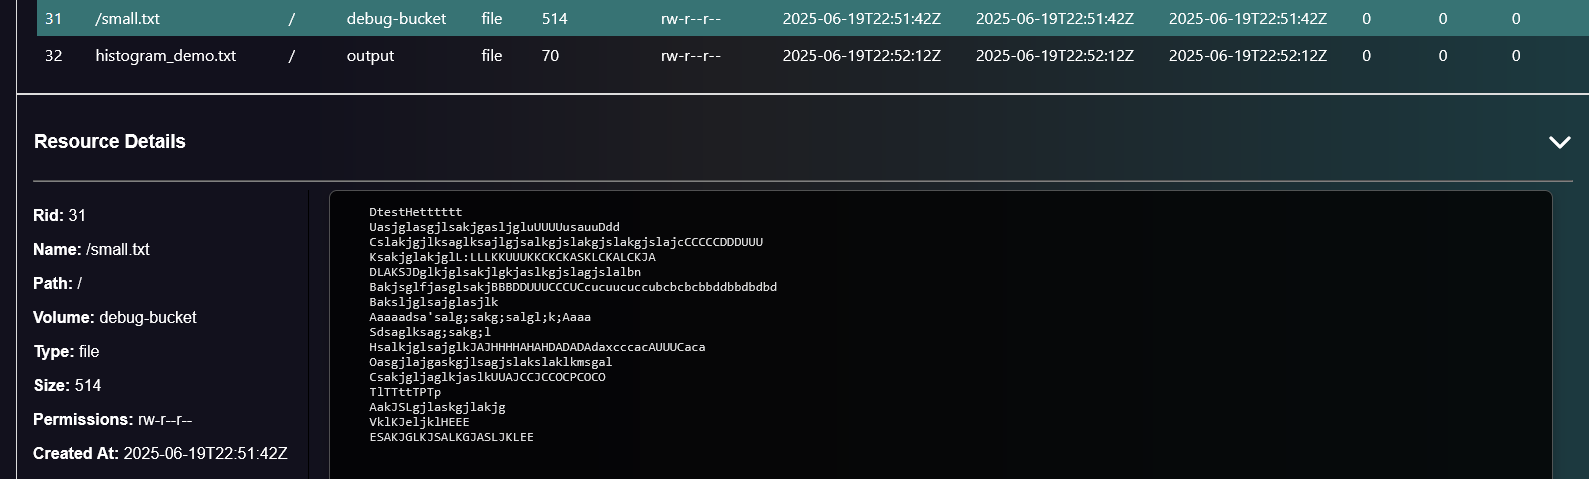
\includegraphics[width=\textwidth]{Images/duckdb_histogram_demo_input.png}
        \caption{DuckDB job input file (preview)}
        \label{fig:exampleduckdb.2}
    \end{subfigure}

    \vspace{1em}

    \begin{subfigure}[b]{0.9\textwidth}
        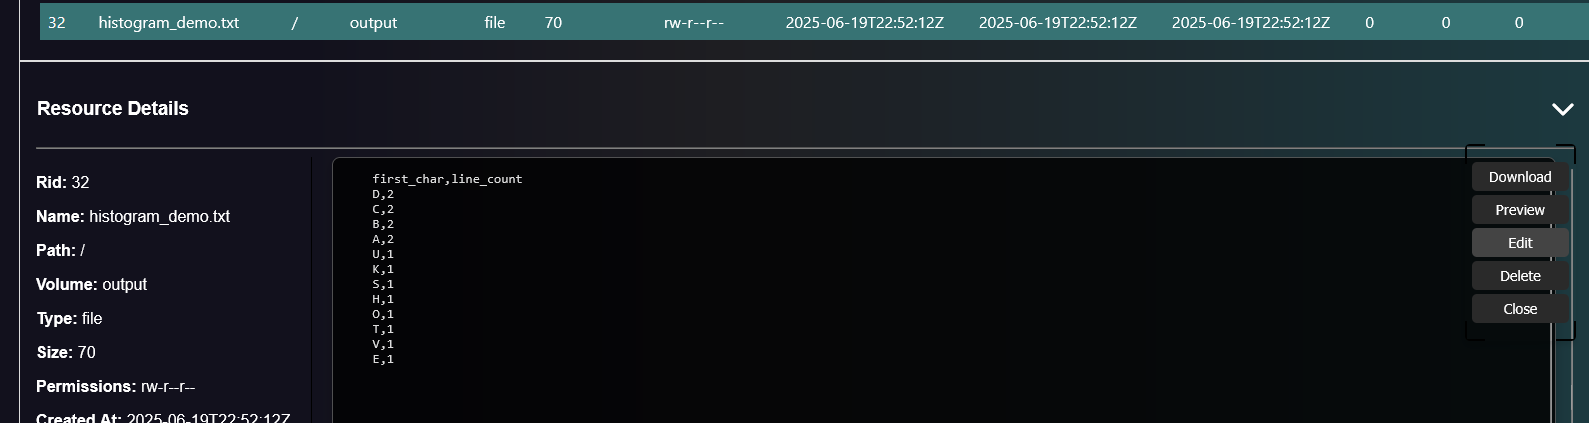
\includegraphics[width=\textwidth]{Images/duckdb_histogram_demo_output.png}
        \caption{DuckDB job result}
        \label{fig:exampleduckdb.3}
    \end{subfigure}
    \caption{DuckDB job: Character frequency histogram from first line characters}
\end{figure}
